% REMEMBER: You must not plagiarise anything in your report. Be extremely careful.

\documentclass{l4proj}
\graphicspath{ {./images/} }
    
%
% put any additional packages here
%
\usepackage{siunitx}
\usepackage[table,xcdraw]{xcolor}
\usepackage{tablefootnote}
\begin{document}

%==============================================================================
%% METADATA
\title{Digital Multilingual News Surveillance and Classification System}
\author{Adam Fairlie}
\date{March 06, 2023}

\maketitle

%==============================================================================
%% ABSTRACT
\begin{abstract}
    Current digital disease surveillance systems lack diversity in their data collection systems, and require results to be translated into English before processing. We developed a more robust data collection system which integrates various types of online data into one system, as well as a web interface to manage the system and view results. Various multilingual machine learning techniques were explored and a classifier to assign categories to incoming multilingual articles was trained and integrated into the collection system. The classifier achieves 89.4\% accuracy on collected data
\end{abstract}

%==============================================================================

% EDUCATION REUSE CONSENT FORM
% If you consent to your project being shown to future students for educational purposes
% then insert your name and the date below to  sign the education use form that appears in the front of the document. 
% You must explicitly give consent if you wish to do so.
% If you sign, your project may be included in the Hall of Fame if it scores particularly highly.
%
% Please note that you are under no obligation to sign 
% this declaration, but doing so would help future students.
%
%\def\consentname {My Name} % your full name
%\def\consentdate {20 March 2018} % the date you agree
%
\educationalconsent


%==============================================================================
\tableofcontents

%==============================================================================
%% Notes on formatting
%==============================================================================
% The first page, abstract and table of contents are numbered using Roman numerals and are not
% included in the page count. 
%
% From now on pages are numbered
% using Arabic numerals. Therefore, immediately after the first call to \chapter we need the call
% \pagenumbering{arabic} and this should be called once only in the document. 
%
% Do not alter the bibliography style.
%
% The first Chapter should then be on page 1. You are allowed 40 pages for a 40 credit project and 30 pages for a 
% 20 credit report. This includes everything numbered in Arabic numerals (excluding front matter) up
% to but excluding the appendices and bibliography.
%
% You must not alter text size (it is currently 10pt) or alter margins or spacing.
%
%
%==================================================================================================================================
%
% IMPORTANT
% The chapter headings here are **suggestions**. You don't have to follow this model if
% it doesn't fit your project. Every project should have an introduction and conclusion,
% however. 
%
%==================================================================================================================================
\chapter{Introduction}

% reset page numbering. Don't remove this!
\pagenumbering{arabic} 

\section{Motivation}

Diseases can be very quick to spread, travelling quickly between areas and causing harm to many people. It is important to avoid as much harm as possible to have up-to-date information on local disease outbreak risks freely available to members of the public. Traditional methods of disease surveillance can be slow, relying on human experts conducting research and scientific experiments, and often miss coverage of certain diseases or geographic regions. Several digital surveillance systems have been developed to collect real-time information from online sources, such as news articles, which can be used to quickly find and assess the risk of disease outbreaks across the world. This information can allow governments to respond rapidly to any new outbreaks by providing quick risk information to the public and planning for diagnosis, testing and prevention. It is for this reason that many governments are creating systems which incorporate online sources to monitor disease outbreaks, such as the Global Public Health Intelligence Network (GPHIN)\footnote{https://gphin.canada.ca/cepr/aboutgphin-rmispenbref.jsp?language=en_CA} from the Canadian government. \par
Many of these digital surveillance systems are limited in the information they collect. They rely on published news feeds, typically from large established providers in high-resource countries, which retains some of the coverage gap in low-resource areas and minority languages. Other methods of data collection are available which can collect from more sources and are less reliant on the publisher, such as directly scraping and formatting the HTML webpages of news articles. This allows for any source which publishes online news to have its information used in disease risk notifications. Research by \cite{seo2017methods} also suggests that other forms of real-time online data such as search trends and social media posts can be effective in detecting disease outbreaks early.\par

-The pipeline of disease classification often relies on machine translation, which can slow down the overall system and relies on the accuracy of translation systems which may not capture the nuances of multilingual data. Multilingual models have emerged but are not as widely used due to some limitations. Through the task of multiclass topic classification, I will determine the efficacy of multilingual models under the current limitations of labelled annotated data, and use the system to collect my own data to verify real-world effectiveness.

\section{Project Aims}
This project develops a new digital surveillance system for multilingual news data, which aims to improve aspects of an existing system, BioCaster\footnote{http://biocaster.org/}. The new system developed should have the following aspects: 

\subsubsection{News collection system}
The data collection system of BioCaster and many other digital surveillance systems is limited. This project will develop a robust and extensible data collection system which can synthesise data from multiple different sources and source types, allowing for a more extensive selection of online news data to be collected, representing a wider range of public information available including lower-resource countries and minority languages. The project will implement two distinct methods of data collection: RSS\footnote{Really Simple Syndication} feeds and web scraping. It will redevelop an improved version of the current BioCaster data collection system based on RSS feeds so that the current system can integrate into the new system without loss of data sources. A web scraping system will also be developed to extract important information such as article headlines, main bodies and publish dates from a given webpage.
\subsubsection{Multilingual news classification}
The project will explore multilingual classifier models, through the task of multiclass classification. Experiments will be conducted on techniques in multilingual classification and a dataset will be gathered using the data collection system, which will be used to train a multilingual classifier model. This classifier will integrate into the data collection system, allowing for classification of incoming news data without the need for machine translation. The classifier should achieve high accuracy on a dataset which represents the news the data collection system will retrieve.
\subsubsection{Data storage and visualisation} The collected news data will be stored in structured form in a database. The information will then be used to produce real-time visualisations of collected data, aggregated into useful statistics, graphs and charts, so that data collected can be observed and analysed. These visualisations should include information on the source countries and languages of collected data, the methods of collection used to retrieve the data and the category distributions of news articles. The system should frequently update and be easy to understand.
\subsubsection{Web interface} A web interface will be developed so that the data collection system can be easily managed, including enabling/disabling data sources, and adding and removing sources. The system should display the last time sources have collected new data, allowing for the highlighting of stale sources which can be removed to save resources. The interface should be responsive and easy to use and understand.

\section{Chapter outline}
This chapter outlines the motivation behind the project and some of the key goals. Future chapters will provide more detail on the exact system design and implementation, and evaluate how effectively the system meets these proposed goals. The paper structure is as follows:
\begin{itemize}
\item \textbf{Chapter 2} covers research into existing digital surveillance systems, real-time data visualisation systems and the currently available news datasets and approaches to news article classification. 
\item \textbf{Chapter 3} covers the high-level system design of the overall system and its components, and describe the plan for experiments related to multilingual multiclass news article classification.
\item \textbf{Chapter 4} covers the exact implementation details of the system, and the exact process for data collection and training of multilingual classifier models.
\item \textbf{Chapter 5} presents the results of the evaluations to consider whether the system achieves its goals. These evaluations are the usability tests for the visualisation and web interface, and the results of training the multilingual classifiers.
\item \textbf{Chapter 6} summarises and reflects on the project and considers future work which could be carried out to extend or improve certain aspects.
\end{itemize}

%==================================================================================================================================
\chapter{Background}
\section{Digital news surveillance systems}

Several digital news surveillance systems exist for different purposes, including research systems for public health monitoring and commercial systems designed for businesses to track information related to their brand. This section considers some of these systems and how they operate.

\subsection{BioCaster}
This project reworks and extends some of the functionality currently used in BioCaster\footnote{http://biocaster.org/}. BioCaster is a digital news surveillance system currently developed by a research team from the University of Cambridge and McGill University, which uses real-time online news data to rapidly create and display risk alerts for disease outbreaks across the world. \par
\begin{figure}[h]
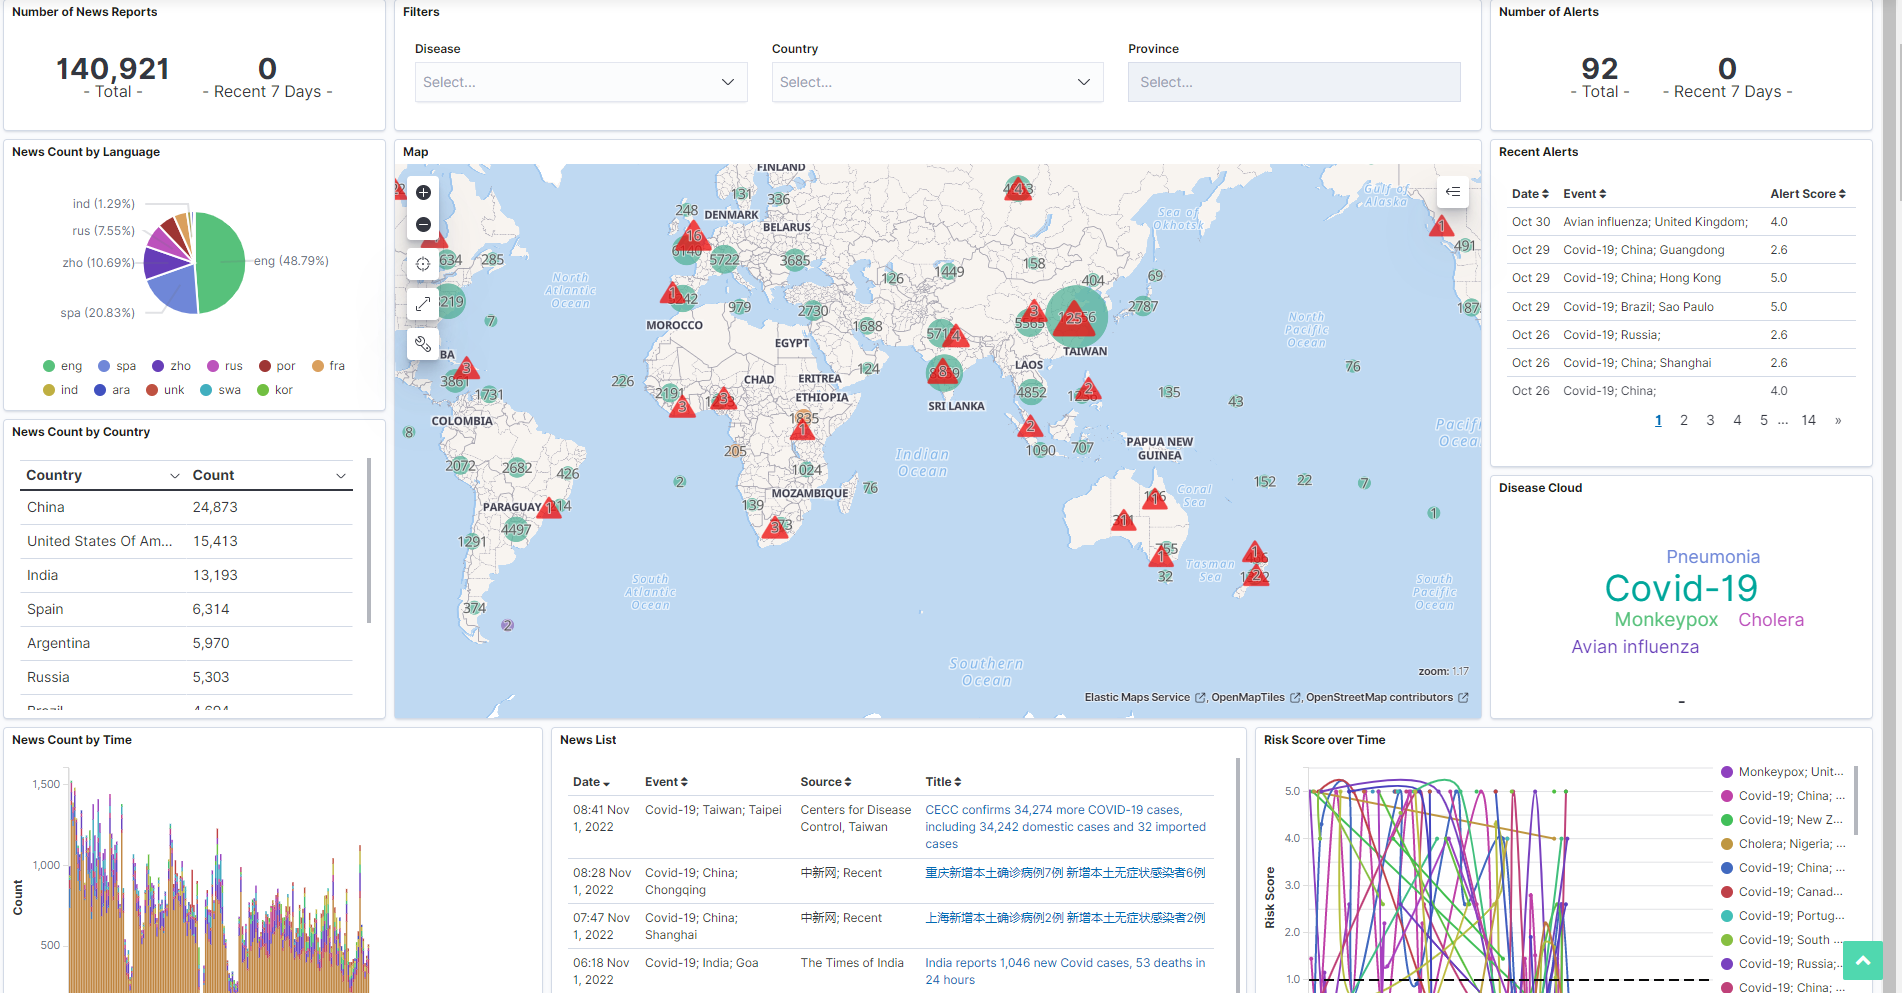
\includegraphics[width=\textwidth]{/biocaster_interface.png}
\caption{The BioCaster visualisation (from http://biocaster.org)}
\label{fig:biocaster_visualisation}
\end{figure}
 The BioCaster system collects news articles through a variety of RSS (Really Simple Syndication) feeds across different languages including English, French and Mandarin \citep{collier2008biocaster}. It uses a machine translation server to translate the headlines and article descriptions into English, and various machine learning and rule-based models to filter the English-language data to remove all irrelevant (not disease-related) articles and collect specific details which are used to create a risk alert. These alerts are displayed in a visualisation on the website. A full diagram of the BioCaster system architecture is shown in Figure \ref{fig:biocaster_architecture}. 
 \begin{figure}[h]
 \centering
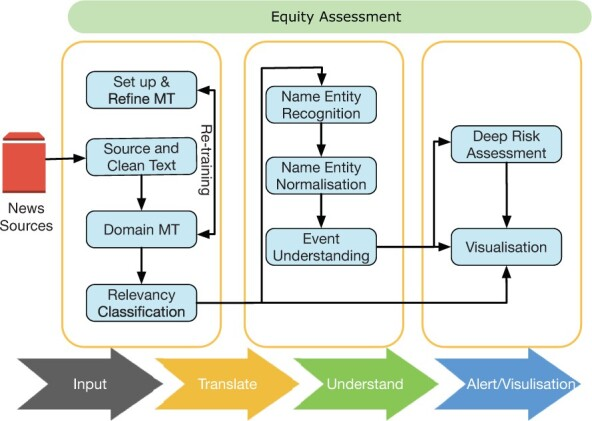
\includegraphics[width=0.75\textwidth]{/biocaster_diagram.jpg}
\caption{The full architecture of the current BioCaster app. Image obtained from \cite{meng2022biocaster}}
\label{fig:biocaster_architecture}
\end{figure}
\par
\subsubsection{Data collection} \hfill \par
The current BioCaster data collection method is dated: it has not been updated in many years and only collects data through RSS feeds, by running a Perl script once per hour to receive updates \citep{collier2008biocaster}. This requires a news source to publish and maintain a feed for its data to be used in the system. These feeds are provided by a limited number of news sources, which are typically larger and written in high-resource languages and countries, where data is not as underrepresented. As  This greatly limits the amount of data which can be extracted, particularly from smaller sources in underrepresented countries and minority languages, and as RSS technology is becoming more outdated and falling out of use, the data available for use in surveillance is continuing to diminish in the current system. The data collected from RSS feeds is also limited to a headline and in some cases a short or medium-length description of article content. This provides limited information to models in later stages of the process for performing relevance classification and risk alert creation tasks. \par
This project will update the BioCaster RSS collection system, as well as add a module for using web scraping to collect news articles from webpage HTML. The system will be designed so that it is easily extensible to other sources of data which may be more prominent in different countries than traditional news, such as social media posts. This also allows for entire article text to be collected instead of just the headline and a short description, which may allow for a richer understanding of the news content and more effective performance in ML tasks.
\subsubsection{Visualisation} \hfill \par
The BioCaster visualisation is made of many components. Its central component is a diagram of the world populated with red and green icons which show the area, range and severity of disease outbreak events. There are many other visualisation components such as information on the number of reports and alerts and a pie chart representing the language distribution of reports. The widget also contains a filter bar, where each of these visualisations can be filtered by disease, country or province, where the data will update in real-time to reflect the filtering. 


\subsection{HealthMap}
HealthMap\footnote{https://www.healthmap.org/en/} is another digital disease surveillance system, created by PhHD's John Brownstein and Clark Freifeld. It provides a world map with location-based disease markers for each country, using RSS data and sources gathered by health experts. \par
\begin{figure}[h]
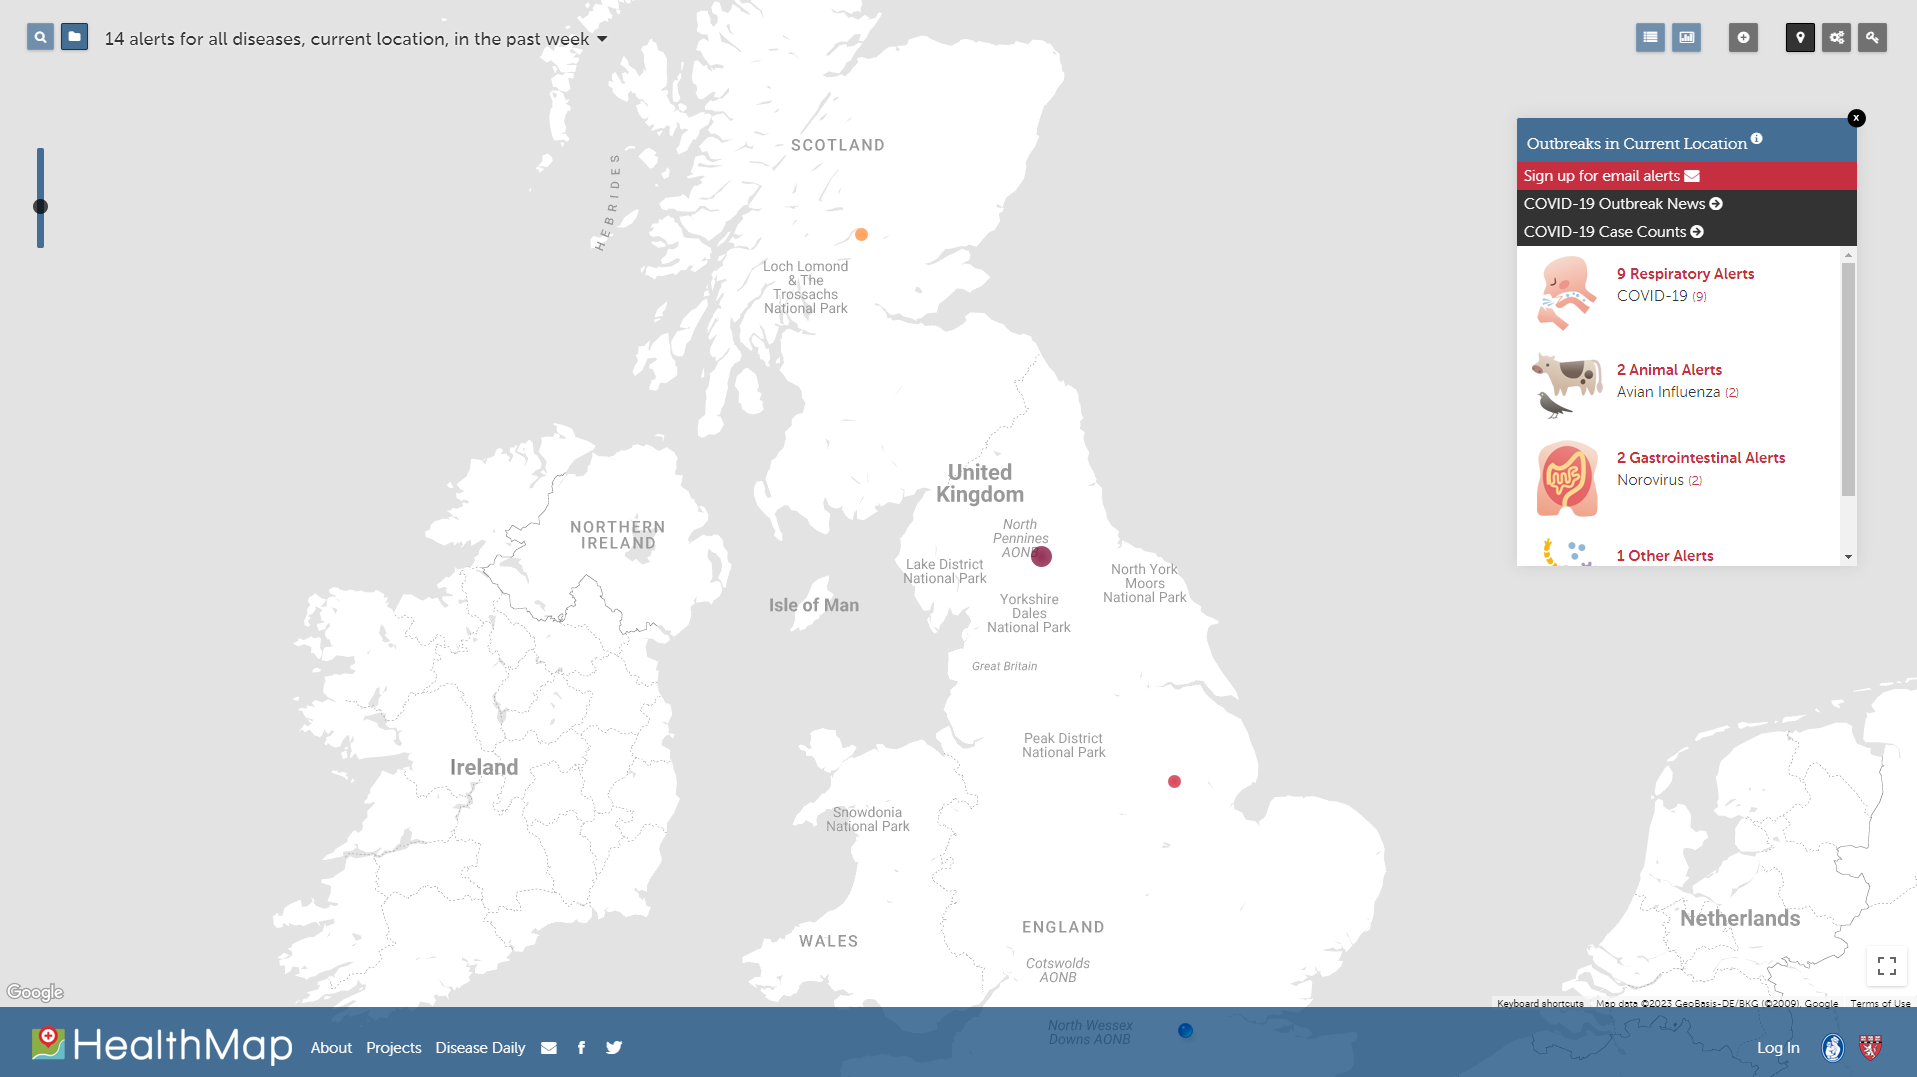
\includegraphics[width=\textwidth]{/healthmap.png}
\caption{HealthMap web interface (from https://www.healthmap.org/en/)}
\label{fig:healthmap_visualisation}
\end{figure}
\textbf{(TO BE COMPLETED)}


\subsection{Other Systems}
\textbf{(TO BE COMPLETED, e.g. Meltwater)}


\section{Multiclass News Article Classification}
\subsection{Datasets}
\textbf{(TO BE COMPLETED)}
-Valurank news classification huggingface. Chosen because the categories and article distribution is good.
\subsection{Models}
\textbf{(TO BE COMPLETED)}


%==================================================================================================================================


\chapter{Design}
\section{Design Principles}
The system architecture was designed with consideration towards a few key software design principles and concepts. The main influences and aims of the overall system design are:
\begin{itemize}
    \item \textbf{Separation of concerns: } Each individual component of the system is given its own module which encapsulates its main functionality and interaction with other modules. This also means that components could possibly be re-used in future projects.
    \item \textbf{Configurability: } The system is designed to give the user as much choice as possible. The system can read a config file which allows the user to control many aspects of the system, such as whether a local or cloud database is used and the maximum number of active sources which are loaded. In addition, individual components are designed so that they can easily be switched out if new components are developed.
    \item \textbf{Extensibility: } Modules of the system which can have implementations changed or new versions created are designed so that this process is as easy as possible, abstracting the consistent functionality of the module into a superclass that new components will inherit from. As previously discussed, social media data has been shown to be a powerful indicator of disease outbreaks, so this system could be extended by adding a social media crawler, for example.
\end{itemize}

\section{System Overview}
Figure \ref{fig:system_overview_diagram} shows a diagram of the overall system architecture.
 \begin{figure}[h]
\centering
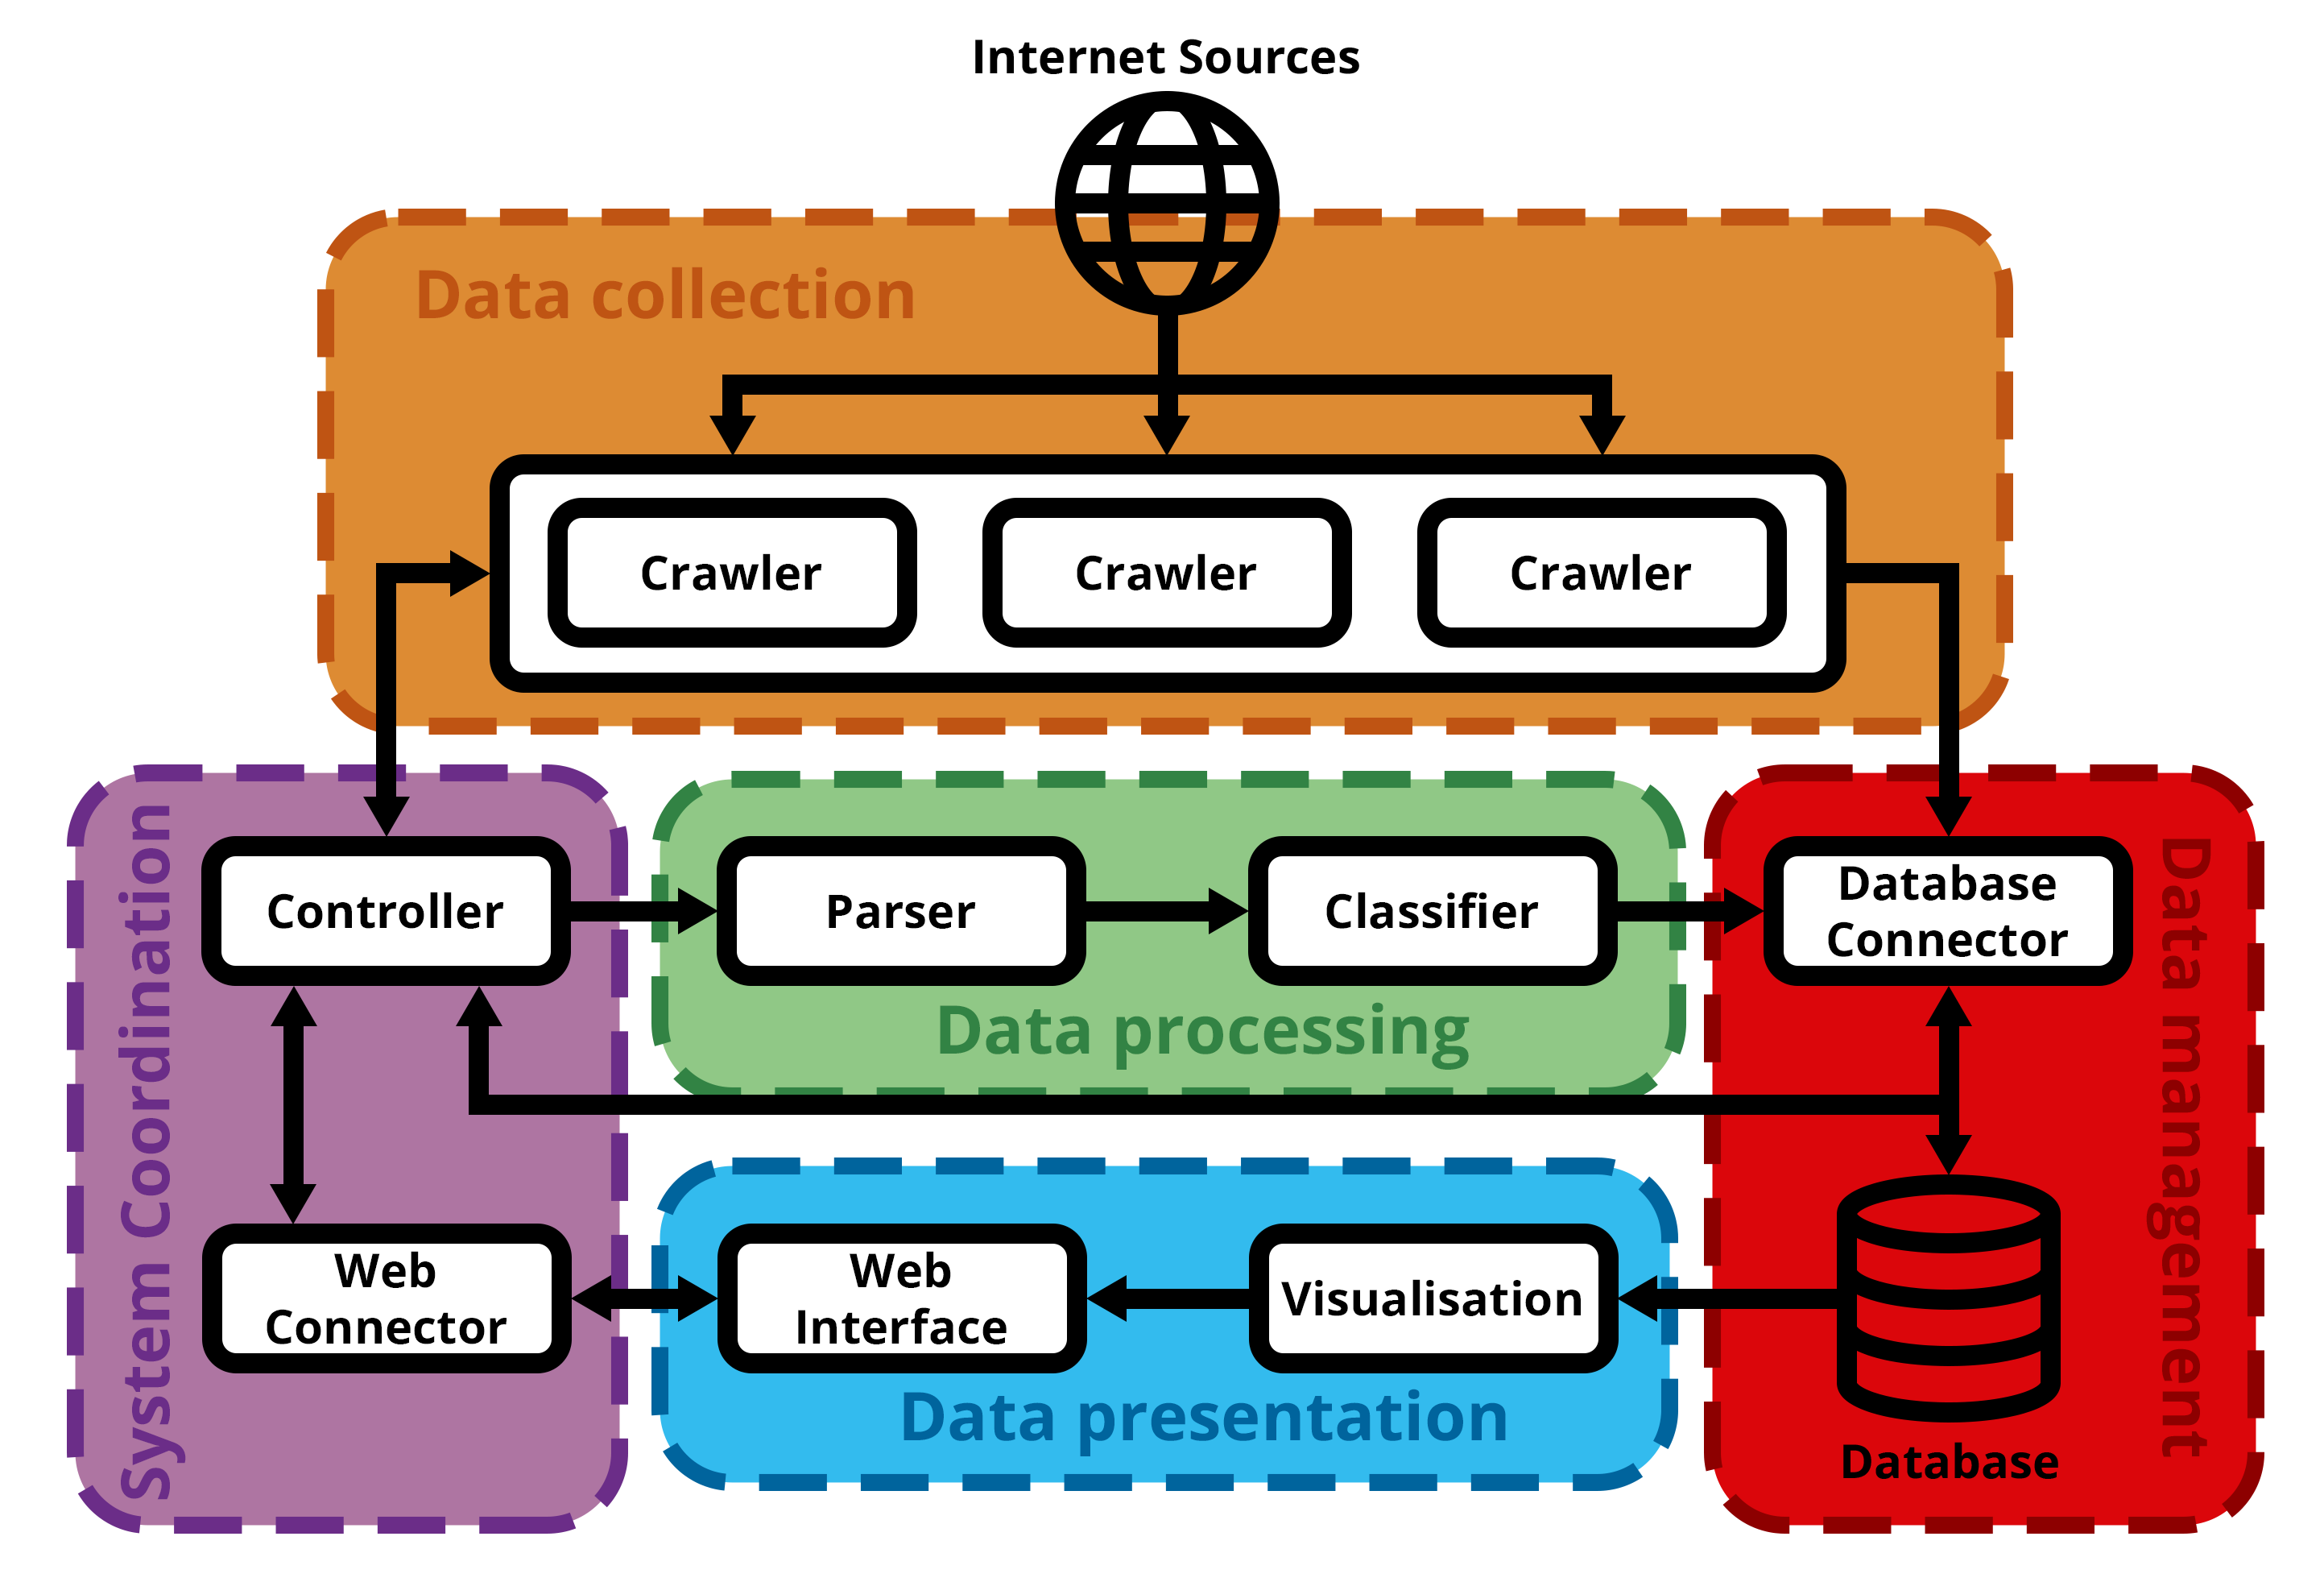
\includegraphics[width=\textwidth]{images/system_overview_diagram.png}
\caption{The overview of the system architecture for this project, showing the different modules and interactions between them. Each module is contained in a box. Arrows indicate the transfer of data between modules (e.g. A -> B means module B receives data from module A. The larger, coloured boxes indicate different subsystems. }
\label{fig:system_overview_diagram}
\end{figure}
\par
\subsection{Modules}
The overall system is designed so that modules can be swapped out and replaced or added into the system in order to cover different sources of online data. In this project, the system and its modules will be designed to gather news articles from RSS feeds and news websites. The purpose of each module in the overall system is as follows:
\begin{itemize}
    \item \textbf{Crawler: } Connect to an internet source (in this case, an RSS feed or website) and obtain a list of URL's to be parsed for the system (in this case of news articles).
    \item \textbf{Article parser: } Parse the given list of URLs, mining the page source content for details (in this case, Headline, publish date etc.)
    \item \textbf{Classifier: } Pass each article through a machine learning model in order to assign it a category (in this case, each news article is given a topic).
    \item \textbf{Database connector: } Provide an interface to allow the system to access the external database.
    \item \textbf{Database: } Permanently store the collected and classified data, and the crawlers, in a structured form.
    \item \textbf{Visualisation: } Present the collected and aggregated data in a number of graphs, charts and statistics for monitoring and interpretation
    \item \textbf{Web interface: } Allow administrators to see the visualisation and to manage the active crawlers.
    \item \textbf{Web connector: } Provide an interface for communication between the management website and the scraping system.
    \item \textbf{Controller: } Initialise crawlers from the sources stored in the database. Send the parsed articles to the classifier and communicate with the web interface (send updates and receive instructions).
\end{itemize}


\section{Data collection}
The data collection system crawls an internet source for all URLs which can possibly contain useful information. In this project, we are concerned with finding the URLs of news articles from a news website or RSS feed. To be appropriate in a disease surveillance system, the data should be updated in near real-time so outbreaks can be quickly understood and responded to.

\subsection{Crawler}
The crawler is the first stage of the data collection process. It represents one individual data source collected in the system, either an RSS feed or a website which is scraped for articles. Crawler objects are stored as a row in a data table of sources. The objects are instantiated from information given by the web interface when a new source is added, or from an existing source in the database. The responsibilities of a crawler are:
\begin{itemize}
    \item Instantiate itself from information stored in the database or given by the web interface.
    \item Add itself to the database if it did not already exist.
    \item Establish a connection with an internet source, in order to receive information.
    \item Create a list of potential sources of data to be parsed (a list of article URLs).
    \item Update its state when it has received new data or instructions.
    \item Update the database with its new state (e.g. delete itself or update its last scrape time).
\end{itemize}
An abstract crawler class encapsulates most of the functionality of this module, handling all communication between other modules. Any concrete crawler implementations (in this project, there are 2: RSS feed crawler and Web crawler) only have to create a method to crawl specific types of data from the internet and use it to update the last scraped date, as well as override the constructor to add its source type. A full diagram of crawler functionality is shown in Figure \ref{fig:crawler_diagram}
 \begin{figure}[h]
\centering
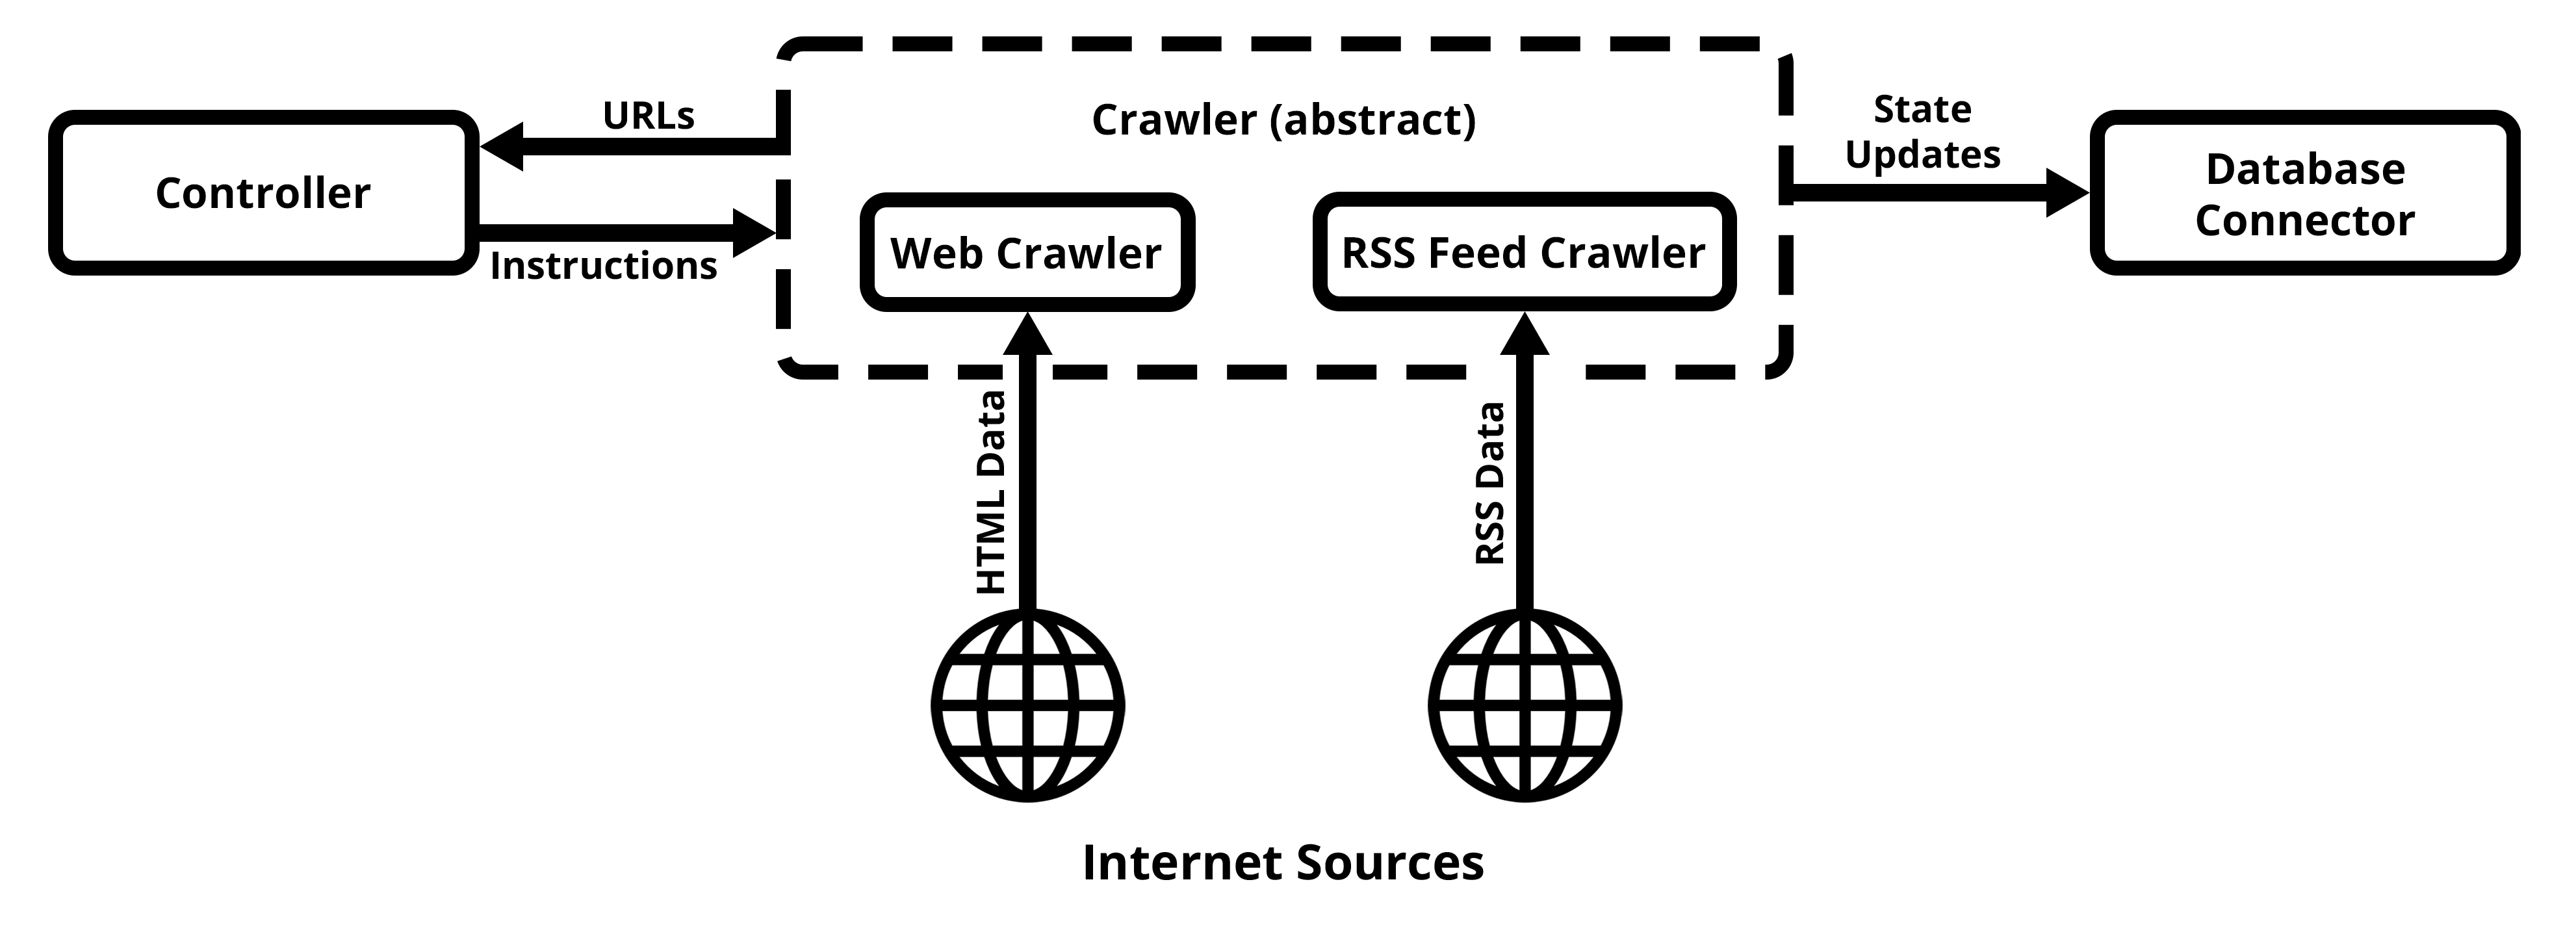
\includegraphics[width=\textwidth]{images/Crawler-diagram.png}
\caption{The overview of the inputs and outputs of the crawler system. The diagram shows the concrete Web Crawler and RSS Feed Crawler implementations being encapsulated by the abstract crawler class, which handles interactions with other modules. The concrete classes each collect a different type of data from the internet sources.}
\label{fig:crawler_diagram}
\end{figure}


\section{Data Processing}
The data processing system creates structured data from internet sources, converting unclean data such as an RSS feed or the HTML of a webpage into a formatted news article with a headline and article body and associated data. It also attempts to understand the data by assigning a category to the incoming articles. The data processing subsystem should be able to process data at a high volume from sources in 10 different languages: English, French, Spanish, Portuguese, Russian, Indonesian, Mandarin, Korean and Arabic. When data is processed, it will be added to the database so it can be used in visualisation.

\subsection{Parser}
The parser receives as input a combined list of URLs from the crawlers and for each URL, will retrieve the page HTML and use it to extract details about the page (in this case, the pages will be news articles) which can be inserted into the database. The article URLs will be shuffled randomly before parsing to avoid very fast repeated requests to the same host, which smaller sources may not be able to easily handle. The parser assumes that news sources are monolingual to avoid language detection wherever possible, but will attempt to detect the language if parsing is incorrect. After this process is complete, the parser sends the parsed data to the classifier to assign the article a topic. The information required from a news article for this project, which the parser will attempt to scrape, is:
\begin{itemize}
    \item Article headline
    \item Article body
    \item Publish date
    \item Language
\end{itemize}
 An abstract parser class handles all communication with other modules. Any concrete parser implementations (such as the article parser in this project) only have to implement a specific method for crawling a list of given URLs and retrieving structured data from the URLs and returning a final list. A full diagram of parser functionality is shown in Figure \ref{fig:parser_diagram}
 \begin{figure}[h]
\centering
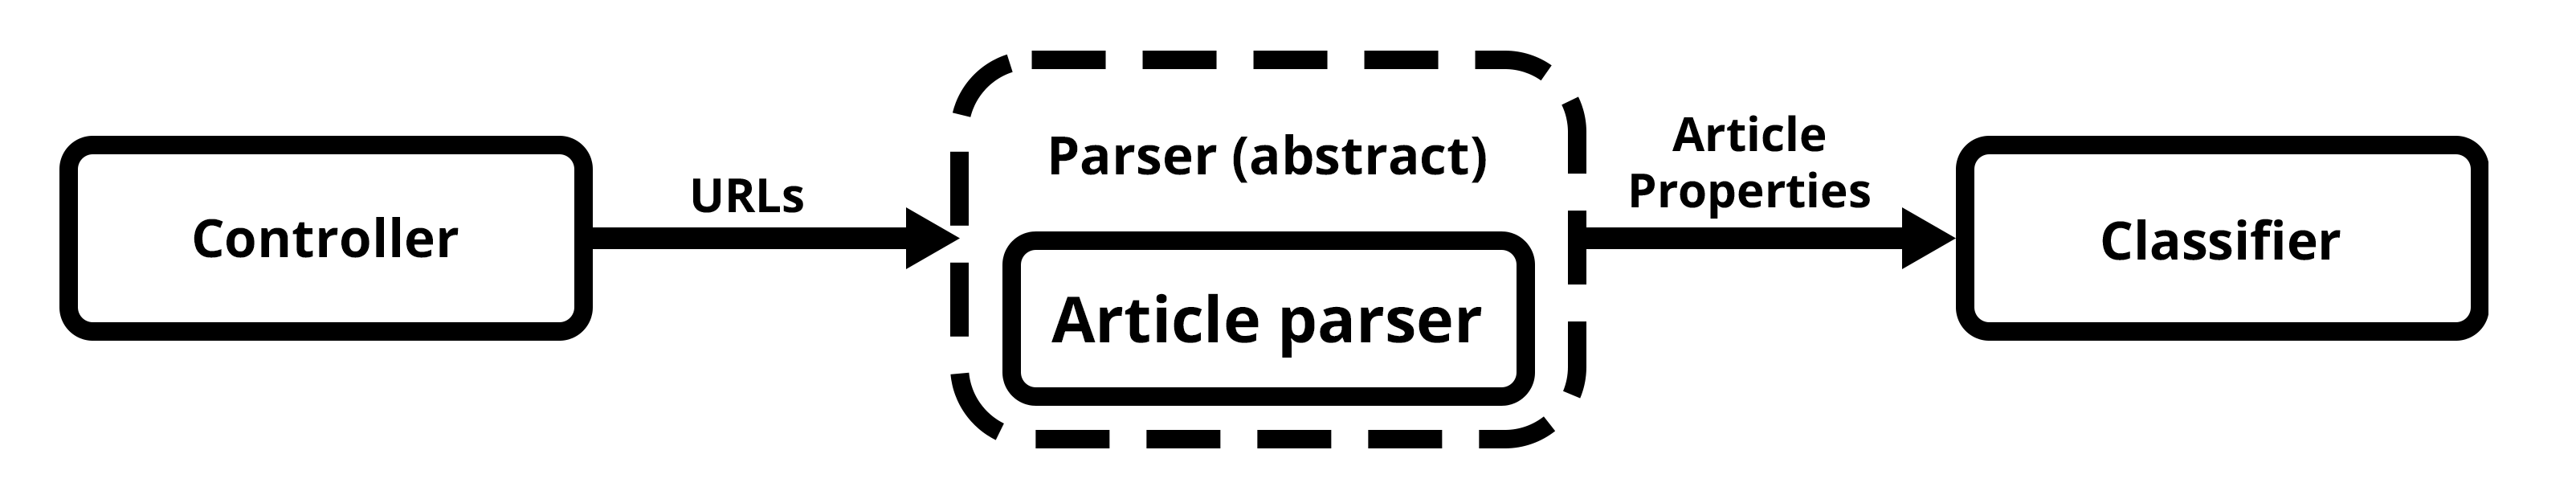
\includegraphics[width=\textwidth]{images/Parser-diagram.png}
\caption{The overview of the inputs and outputs of the parser system. The diagram shows the concrete article parser implementation being encapsulated by the abstract parser class, which handles interactions with the controller and classifier.}
\label{fig:parser_diagram}
\end{figure}

\subsection{Classifier}
The classifier receives a list of parsed articles, with features extracted. It then performs any necessary data preparations and tokenization before feeding the articles through a trained classifier model to assign a category to each news article (e.g. Sports, Entertainment). In this project, the classifier module will use a pre-trained BERT-based classifier model loaded from a file and will tokenize and classify the concatenated article headline and body. The parsed articles with topics will be sent to the database connector and inserted into the database. \par
An abstract classifier class handles communication with other modules and batching of input data. To create a concrete classifier implementation, we would have to implement:
\begin{itemize}
    \item A constructor which properly initialises the model and any tokenizers.
    \item A method which preprocesses a list of input data.
    \item A method which receives an input batch and outputs a list of corresponding classification labels.
\end{itemize}
A full diagram of classifier functionality is shown in Figure \ref{fig:classifier_diagram}
 \begin{figure}[h]
\centering
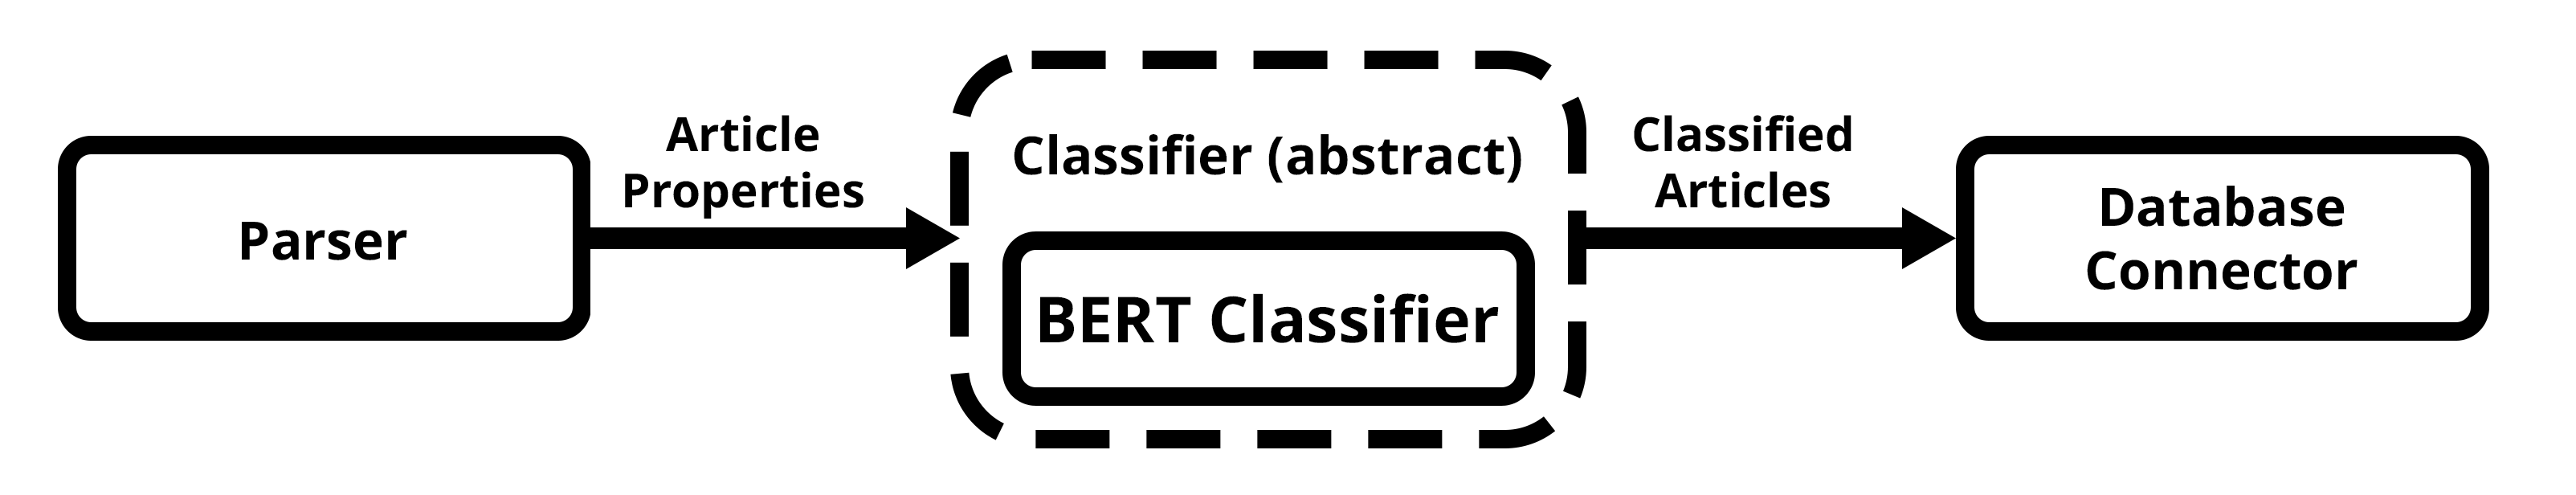
\includegraphics[width=\textwidth]{images/Classifier-diagram.png}
\caption{The overview of the inputs and outputs of the classifier system. The diagram shows the concrete BERT classifier implementation being encapsulated by the abstract classifier, which handles interactions with the parser and database connector.}
\label{fig:classifier_diagram}
\end{figure}

\section{Data Management}
The data management subsystem stores the data (data sources and collected articles) in a permanent form, where it can be shown in the visualisations. The database system should be able to handle many reads (for article duplicate checking) and writes (for inserting new articles) at a high volume. 

\subsection{Database}
For this project, the database will consist of two tables: \textbf{Articles} and \textbf{Sources}. An ER Diagram for the database system is shown in Figure \ref{fig:er_diagram}

\begin{table}[h]
\begin{tabular}{lll}
\hline
\multicolumn{3}{c}{\textbf{Source}}                                                                                                                                      \\ \hline
\textbf{Attribute} & \textbf{Type} & \textbf{Description}                                                                                                                \\ \hline
\textbf{ID}        & Primary Key   & A unique auto-generated source ID.                                                                                                  \\
URL                & Text          & The data source URL (e.g. "https://www.bbc.co.uk/news")                                                                             \\
Name               & Text          & A name describing the source (e.g. "BBC News")                                                                                      \\
Country            & Text (2)      & \begin{tabular}[c]{@{}l@{}}The ISO 3166-1 alpha-2\tablefootnote{https://en.wikipedia.org/wiki/ISO\_3166-1\_alpha-2} code of the country \\ the source originates from (e.g. "GB")\end{tabular}        \\
Language           & Text (2)      & The ISO 639-1\tablefootnote{https://en.wikipedia.org/wiki/List\_of\_ISO\_639-1\_codes} code of the sources main language (e.g. "EN")                                                                         \\
Data Source        & Text          & The type of source this is (e.g. "RSS/Atom feed")                                                                                   \\
Last retrieved     & Date/Time     & The time this source last retrieved new data                                                                                        \\
Active             & Boolean       & \begin{tabular}[c]{@{}l@{}}Whether this source is active \\ (if False, when instantiated the crawler will be disabled)\end{tabular} \\ \hline
\multicolumn{3}{c}{\textbf{Article}}                                                                                                                                     \\ \hline
\textbf{Attribute} & \textbf{Type} & \textbf{Description}                                                                                                                \\ \hline
\textbf{ID}        & Primary Key   & A unique auto-generated article ID.                                                                                                 \\
URL                & Text          & The URL of the article                                                                                                              \\
Headline           & Text          & The article headline                                                                                                                \\
Body               & Text          & The main body of the article                                                                                                        \\
Country            & Text (2)      & The ISO 3166-1 code of the country of the original source                                                                           \\
Language           & Text (2)      & The ISO 639-1 code of the language of the article                                                                                   \\
Published          & Date/Time     & The time this article was published                                                                                                 \\
Retrieved          & Date/Time     & The time this article was retrieved by the scraping system                                                                          \\
Source name        & Text          & The name of the source this article is collected from                                                                               \\
Source type        & Text          & The type of source this article came from (e.g. "Web scraper")                                                                      \\
Category           & Text          & The assigned category of this article (e.g. "Entertainment")                                                                        \\ \hline
\end{tabular}
\caption{List of attributes in the Source and Article tables, with data type and description. Primary key attributes are highlighted in bold. "Text (2)" denotes that this field is a text field which is exactly 2 characters long.}
\label{table:schema}
\end{table}

\subsection{Database Connector}
The database connector provides a connection between the system and the external database, allowing the other modules to send and retrieve the data. In this system, the connector must have functionality for:
\begin{itemize}
    \item Creating the Article and Source tables
    \item Adding new sources and articles
    \item Retrieving stored sources
    \item Deleting sources
    \item Updating sources (enabling/disabling, updating last scrape time)
    \item Searching articles by URL and headline (for duplicate checking) 
\end{itemize}
A full diagram of database functionality is shown in Figure \ref{fig:database_diagram}
 \begin{figure}[h]
\centering
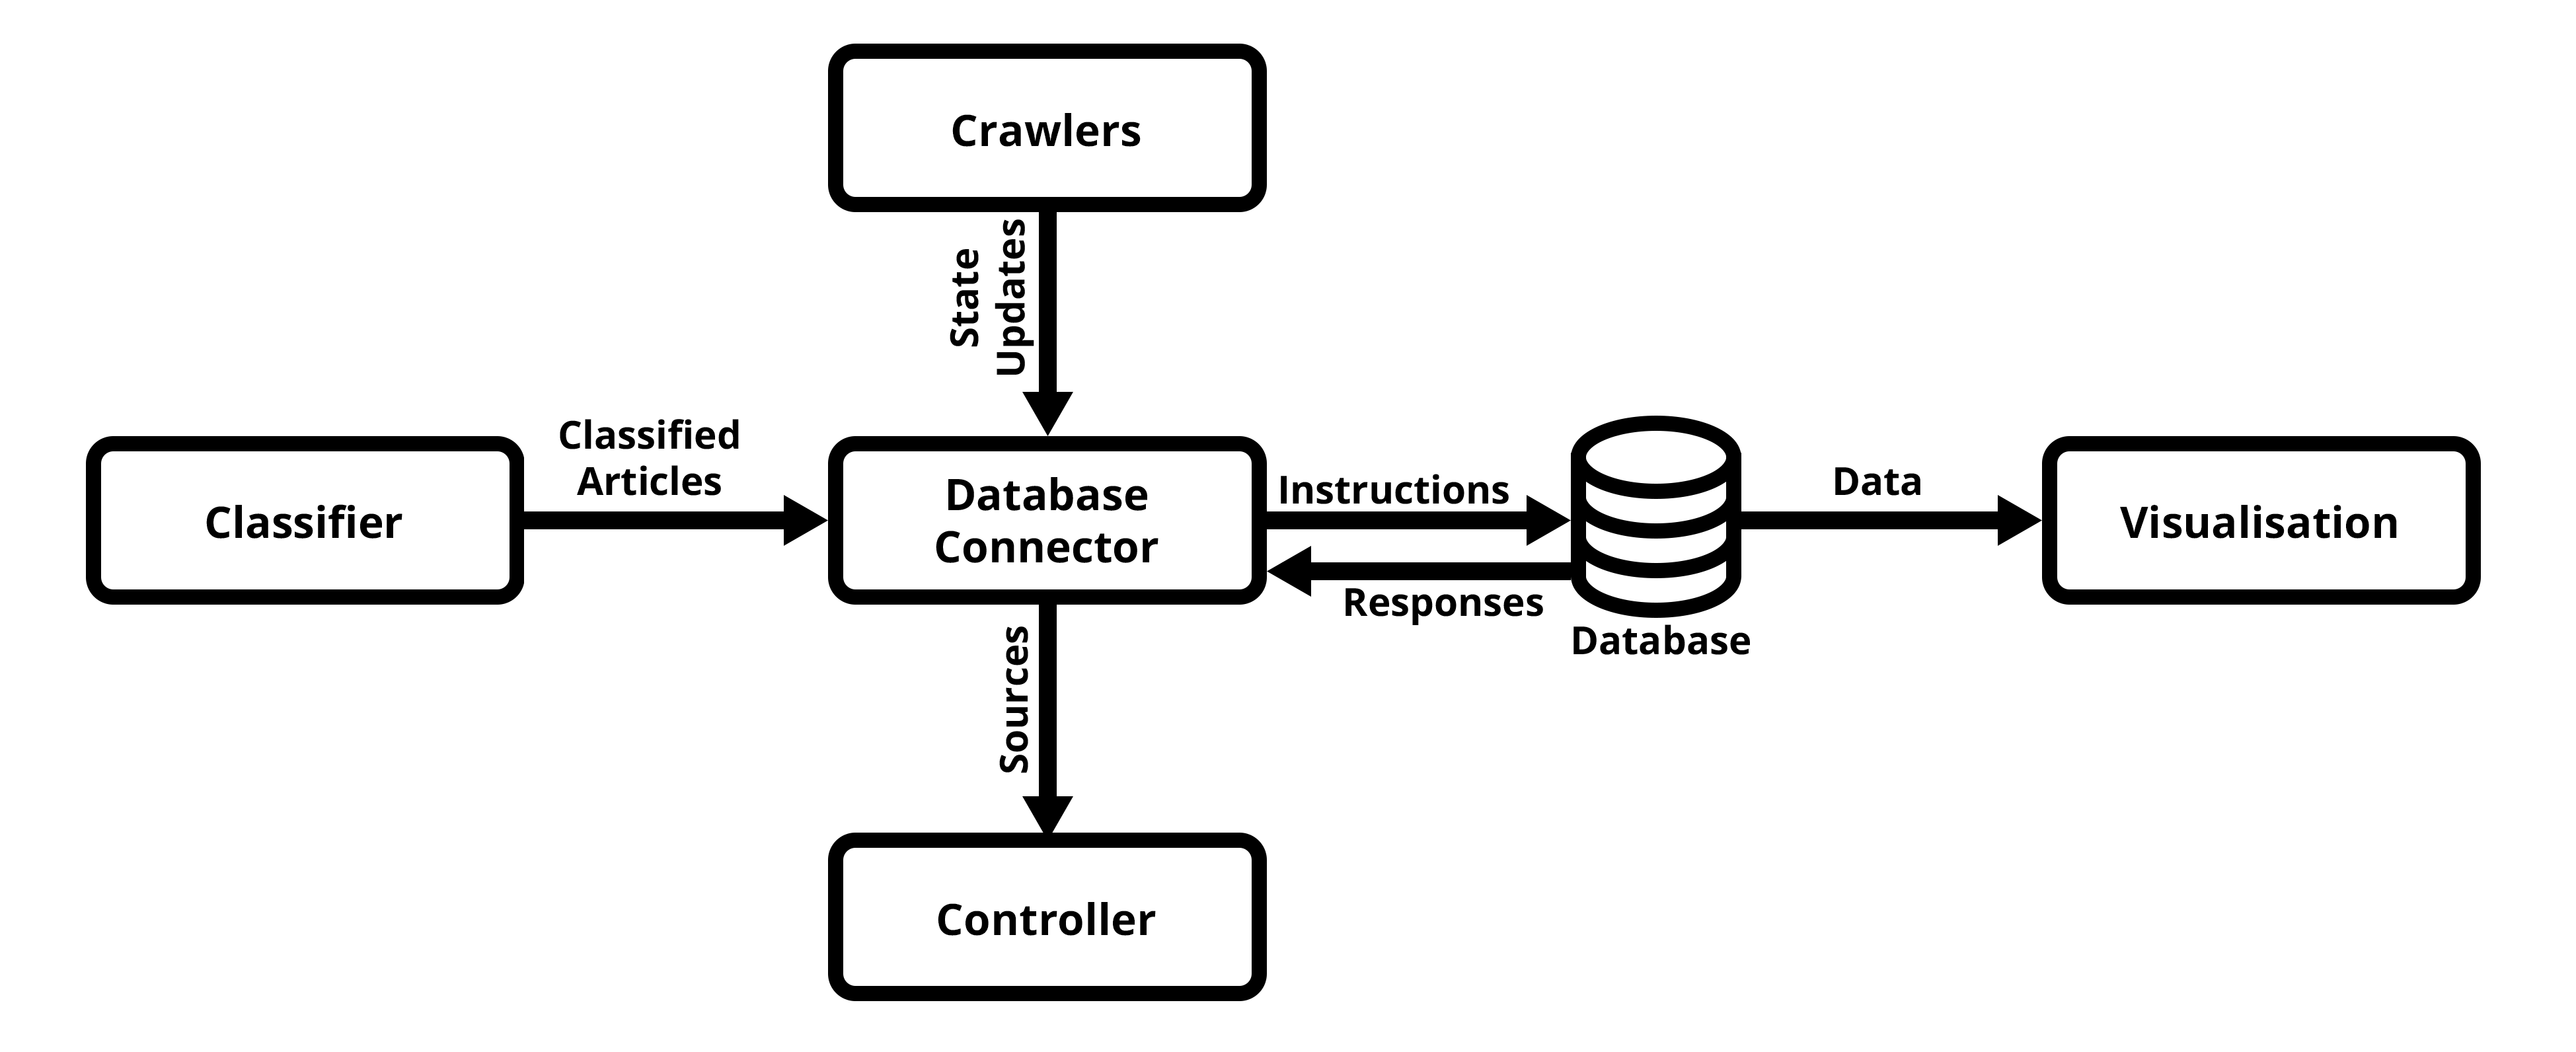
\includegraphics[width=\textwidth]{images/Database-diagram.png}
\caption{The overview of the inputs and outputs of the database and connector.}
\label{fig:database_diagram}
\end{figure}
\section{Data Presentation}
The data presentation subsystem is concerned with creating an easy interface for a user to view, analyse and understand the data collected, as well as easily interact with the system to modify its behaviour. The system should have interfaces which are easy to use and understand and provide useful insight and control on the data collection process.

\subsection{Visualisation}
The visualisation is mainly based on the current BioCaster interface, as shown in Figure \ref{fig:biocaster_visualisation}. This design has been updated to reflect the changes from my project to the current system, including the addition of news article topics and different source types of information retrieved. I also did not have the specific region or disease information to create the alerts seen on the BioCaster interface. Shown in Figure \ref{fig:visualisation-wireframe} is an initial wireframe of the new visualisation: \par
 \begin{figure}[h]
\centering
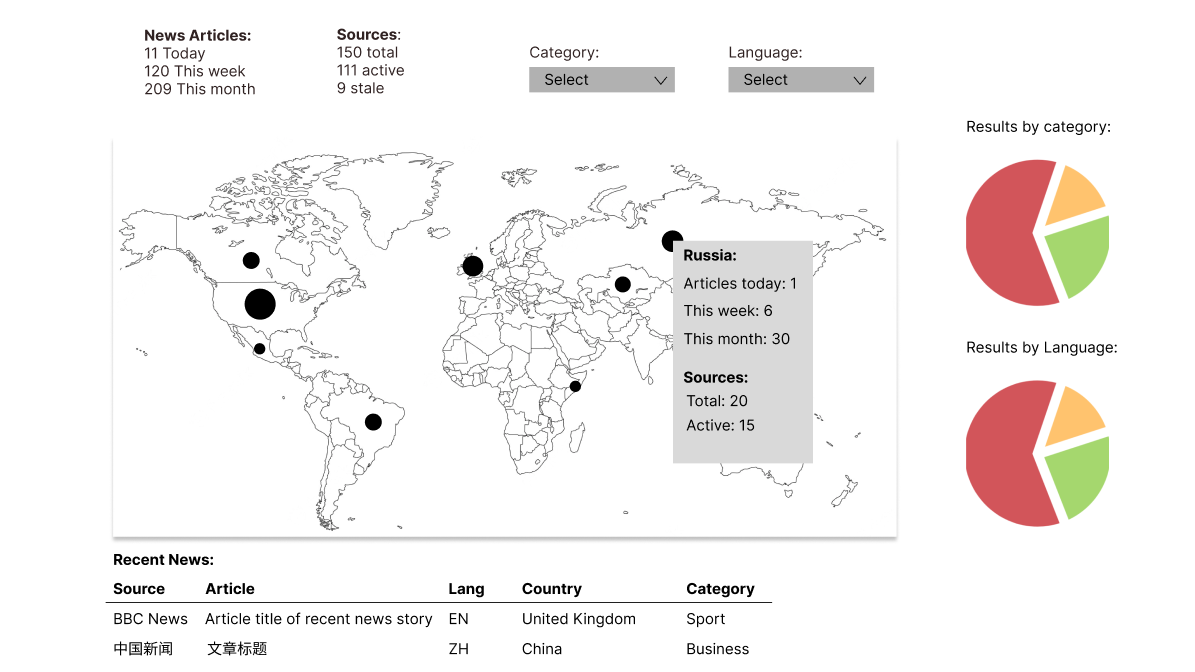
\includegraphics[width=\textwidth]{images/visualisation-wireframe.png}
\caption{The wireframe for the new visualisation.}
\label{fig:visualisation-wireframe}
\end{figure}
After supervisor feedback, more emphasis was placed on filtering by source type. The final visualisation will have the following modules:
\begin{itemize}
    \item A bar for filtering by Category, Language and Source type
    \item A section showing the number of total and active sources
    \item A section showing the number of articles scraped today, this week and this month
    \item Pie charts showing data distribution by source type, language and category
    \item A table showing the most recent articles collected
    \item Time-series data on articles collected over time
    \item A world map showing information per country (number of articles, most common category etc.)
\end{itemize}

\subsection{Web Interface}
The web interface is designed to show the visualisation on a webpage, as well as provide functionality for managing the scraping system. The web interface should provide utility for the following tasks:
\begin{itemize}
    \item Enabling/disabling the entire scraping system
    \item Enabling/disabling individual sources
    \item Deleting individual sources
    \item Adding new sources
    \item Viewing stale sources (this was requested by the BioCaster team)
\end{itemize}
The wireframe for the manage sources page of the web interface is shown in Figure \ref{fig:interface-wireframe} 
 \begin{figure}[h]
\centering
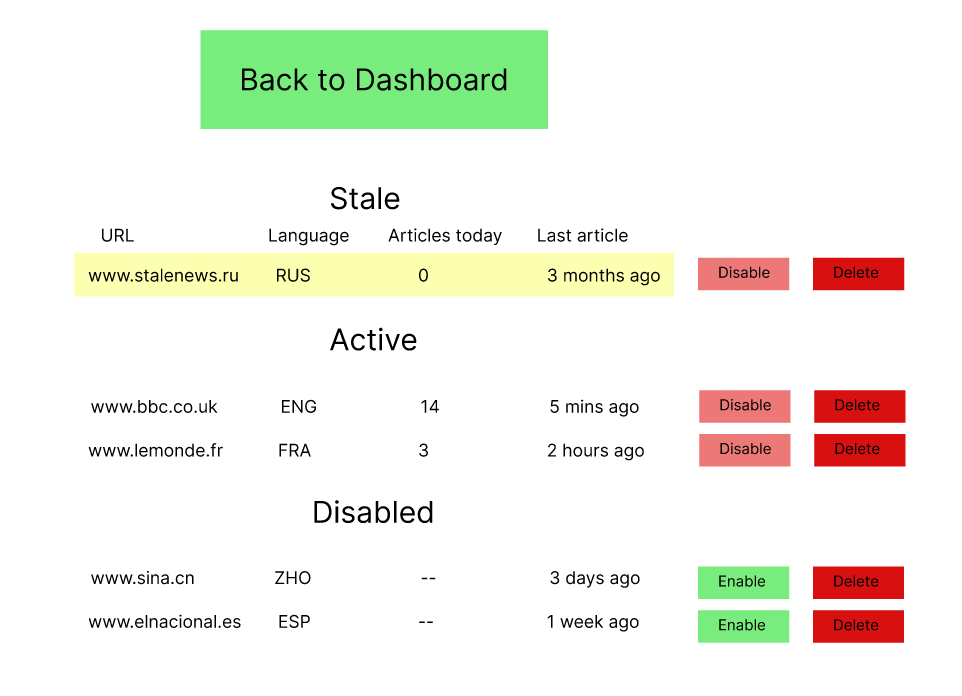
\includegraphics[width=\textwidth]{images/interface-wireframe-sources.png}
\caption{The wireframe for the manage sources page of the web interface.}
\label{fig:interface-wireframe}
\end{figure}

\section{System Coordination}
The system coordination subsystem is responsible for orchestrating the data collection process and connecting subsystems, as well as allowing the interface to communicate with the scraping system.
\subsection{Web Connector}
The web connector provides the interface between the web server and the scraping system. It ensures that the commands performed on the interface are translated into instructions for the controller, which will perform the requested action. These instructions include enabling, disabling, deleting and adding sources, as well as enabling or disabling the entire scraping system. The web interface can also request updates through the web connector, to show the user the most recent information on the most recent scrape times of each source. Figure \ref{web-connector-diagram} shows how the web connector integrates with all other modules.
 \begin{figure}[h]
\centering
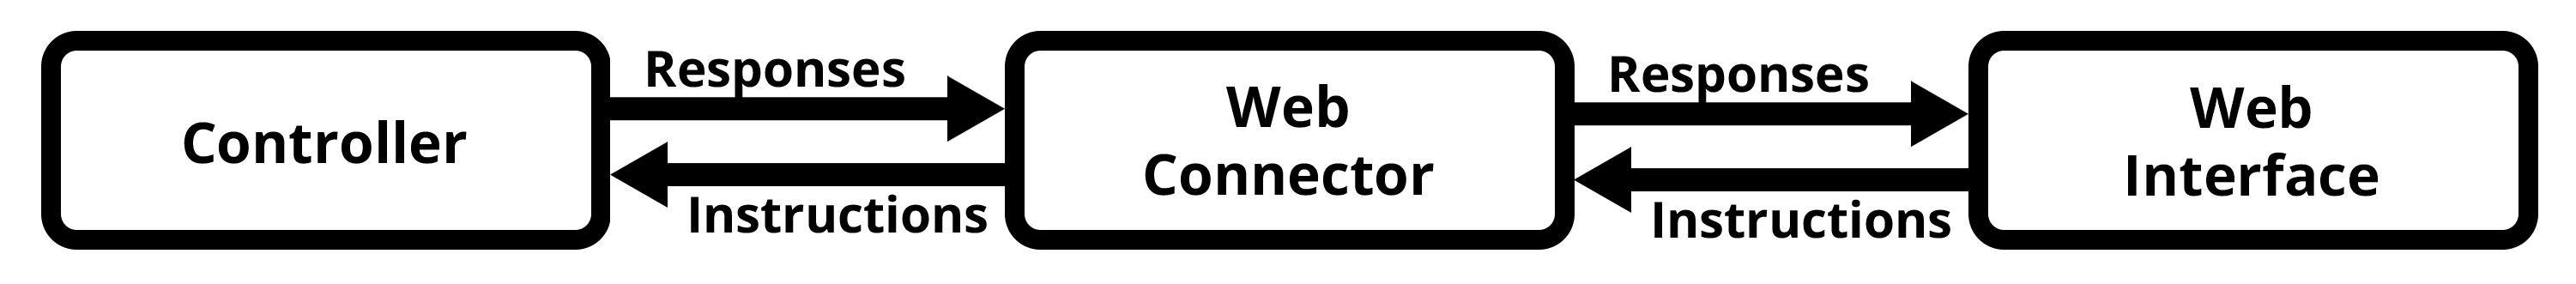
\includegraphics[width=\textwidth]{images/Web-connector-diagram.png}
\caption{The overview of the inputs and outputs of the web connector.}
\label{fig:web-connector_diagram}
\end{figure}

\subsection{Controller}
The controller is the main orchestrator of the system, and is the module called when running the system. It performs the following roles:
\begin{itemize}
    \item Ensures the tables exist in the database.
    \item Receives all sources from the database and instantiates Crawlers.
    \item Instantiates parser and classifier object(s).
    \item Starts the web server for the web interface.
    \item Co-ordinates when the crawlers look for new data.
    \item Sends new crawler data to the parser(s).
    \item Communicates with the web interface through the web connector, sending updates and performing instructions.
\end{itemize}
A full diagram of the controller functionality is shown in Figure \ref{fig:controller_diagram}
 \begin{figure}[h]
\centering
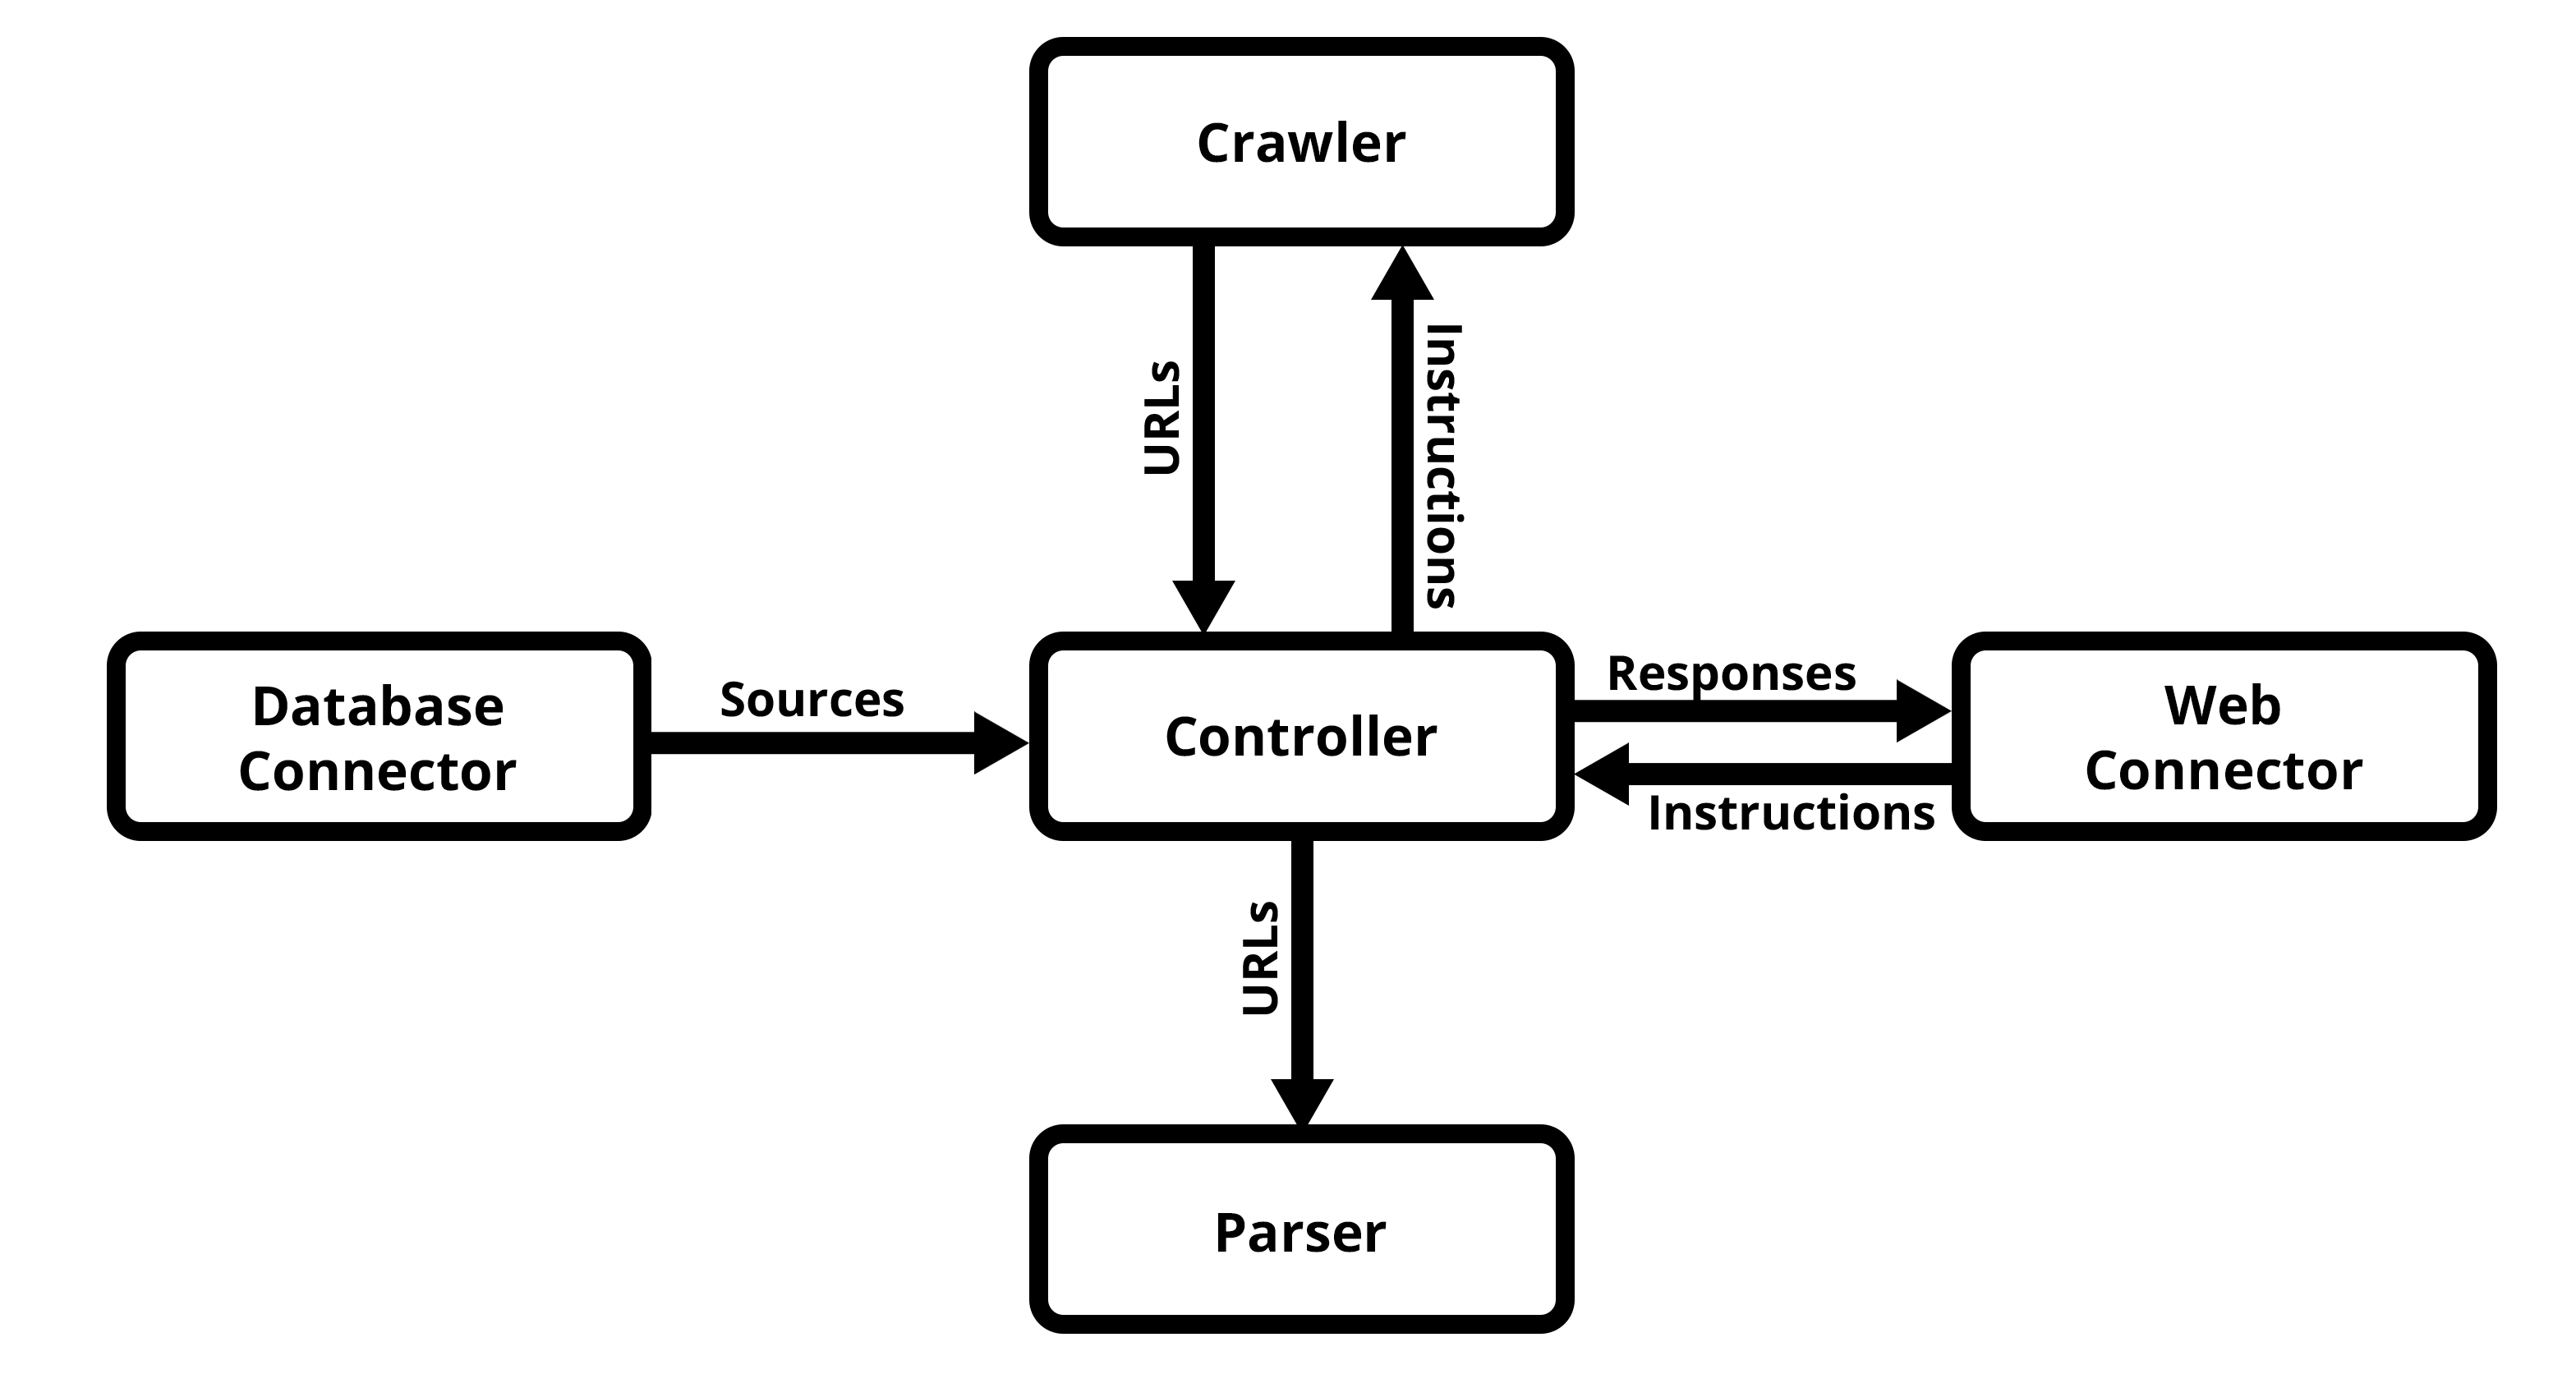
\includegraphics[width=\textwidth]{images/Controller-diagram.png}
\caption{The overview of the inputs and outputs of the controller module.}
\label{fig:controller_diagram}
\end{figure}

%==================================================================================================================================
\chapter{Implementation}
\section{Web Scraping System}
\textbf{(TO BE COMPLETED)}
The main free and open-source technologies for scraping news articles from websites in Python were \emph{Newspaper3K}\footnote{https://github.com/codelucas/newspaper} and \emph{news-please}\footnote{https://github.com/fhamborg/news-please}, which is built on top of Newspaper3K and adds some extra features. Another option considered was \emph{Newscatcher}\footnote{https://newscatcherapi.com/news-api}, but the free API is limited in how many calls can be made and this made it unsuitable for this project. Finally, I considered \emph{pygooglenews}\footnote{https://github.com/kotartemiy/pygooglenews} which provided some promise in using google news to find articles under certain subjects, keywords, languages and regions. For this project, I found it desirable to have better control of the exact sources collected, instead of filtering through keywords and relying on Google's source selection, but a scraper using this library could easily be added to extend the capabilities of the current system. I decided to move forward with the former two libraries and conducted an experiment to compare their capabilities. \par

I compared the features present in each of the two libraries. Notably, Newspaper3K can perform full website scraping in Python, whereas news-please can only do this using its Command Line Interface (CLI). I attempted to scrape 3 articles from each of the 109 previously selected websites, across 10 languages, and compared the number of successful scrapes (without error) and the average speed. The results are shown below: \par 
(Results table to be converted) \par
Newspaper3K scraped 103 of the 109 websites (94.5\%) without error, whereas news-please scraped 102/109 (93.58\%). The average scraping times are similar in both libraries, but Newspaper3K was faster at scraping in 8 of the 10 languages, and average scraping time per article was 14.82\% lower, Based on these factors, I chose to use Newspaper3K for the scraping system.
\section{Database}
\textbf{(TO BE COMPLETED)}
\section{Visualisations and interface}
\textbf{(TO BE COMPLETED)}
The BioCaster visualisation is created using the Elastic software stack\footnote{https://www.elastic.co/elastic-stack/}, where visualisations are created in Elastic Kibana, which automatically generates and updates visualisations from an underlying NoSQL database created using Elasticsearch.

In addition, I chose to change the article density to cover the whole country instead of being a dot, to make the source of the data more visible (so that it does not obstruct the view of other countries) and created a monochromatic green colour map, where darker colours represented more articles retrieved as is common practice in world density maps \citep{ourworldindata_density, ons_density}.

\section{News article classification}

\subsection{Research Overview}
This experiment aims to consider multiclass classification of news articles in different languages, using multilingual models. In particular, this experiment uses articles in six languages: English, French, Spanish, Portuguese, Mandarin and Indonesian. By researching the topics used by the news sources previously collected, as well as the topics used in publicly available news classification datasets, six news topic categories were chosen: Entertainment/Arts, Sports, Politics, Science/Technology, Business/Finance and Health/Welfare. 

In many languages, particularly minority languages, little to no labelled public datasets are available for topic classification of news, meaning models cannot be trained by traditional means. This creates difficulty when trying to perform real-time classification tasks on news written in minority languages, for purposes such as creating disease alerts. We will investigate the efficacy of some techniques and approaches for multilingual document classification, by investigating the following research questions: 
\begin{itemize}
\item How effective is machine translation of English articles into other languages, as a method of upsampling, in increasing the effectiveness of multilingual models? 
\item How effective are models trained on public data (both in English and translated into all 6 languages) when used to classify collected news data directly from sources across the six languages? 
\item What level of performance can be achieved by multilingual models when trained and evaluated on collected articles from sources in each of the six languages?
\end{itemize}

\subsection{Datasets}
\subsubsection{Public data} \hfill \par
The dataset used is a dataset made available on huggingface by \cite{valurankdata}. The data originally consists of 3,722 classified English-language news articles scraped from various online news sources with 7 topic labels: World, Politics, Tech, Entertainment, Sport, Business, Health, and Science. To match the categories being considered in this experiment, articles belonging to the "World" category were dropped, and those belonging to the "Tech" and "Science" categories were merged into a new "Science/Technology" category. An augmented dataset was also created by adding copies of each article translated into each of the other five languages (French, Spanish, Portuguese, Mandarin and Indonesian). Translations were obtained using the Google translate API through the python library \emph{googletrans}\footnote{https://pypi.org/project/googletrans/}. The distribution of topics in the original and augmented datasets is shown in Table \ref{table:valurankstats} and Figure \ref{fig:public_cat_dist}.

\begin{table}[]
\begin{tabular}{llllllll}
\hline
\multicolumn{1}{c}{\textbf{}} & \multicolumn{7}{c}{\textbf{Number of Documents}}                                                                                          \\ \hline
                              & \textbf{Entertainment} & \textbf{Sports} & \textbf{Politics} & \textbf{Science/}   & \textbf{Business} & \textbf{Health} & \textbf{Total} \\
                              & \textbf{}              &                 &                   & \textbf{Technology} & \textbf{}         & \textbf{}       &                \\ \hline
\textbf{Original}             & 485                    & 454             & 442               & 838                 & 461               & 467             & \textbf{3147}  \\
\textbf{Translated}           & 2910                   & 2724            & 2652              & 5028                & 2766              & 2802            & \textbf{18882} \\ \hline
\end{tabular}
\caption{Category distribution of the Valurank news categorization dataset. This table includes the original dataset and the augmented version obtained from adding the translations of each article in each of the other 5 languages.}
\label{table:valurankstats}
\end{table}

\begin{figure}[h]
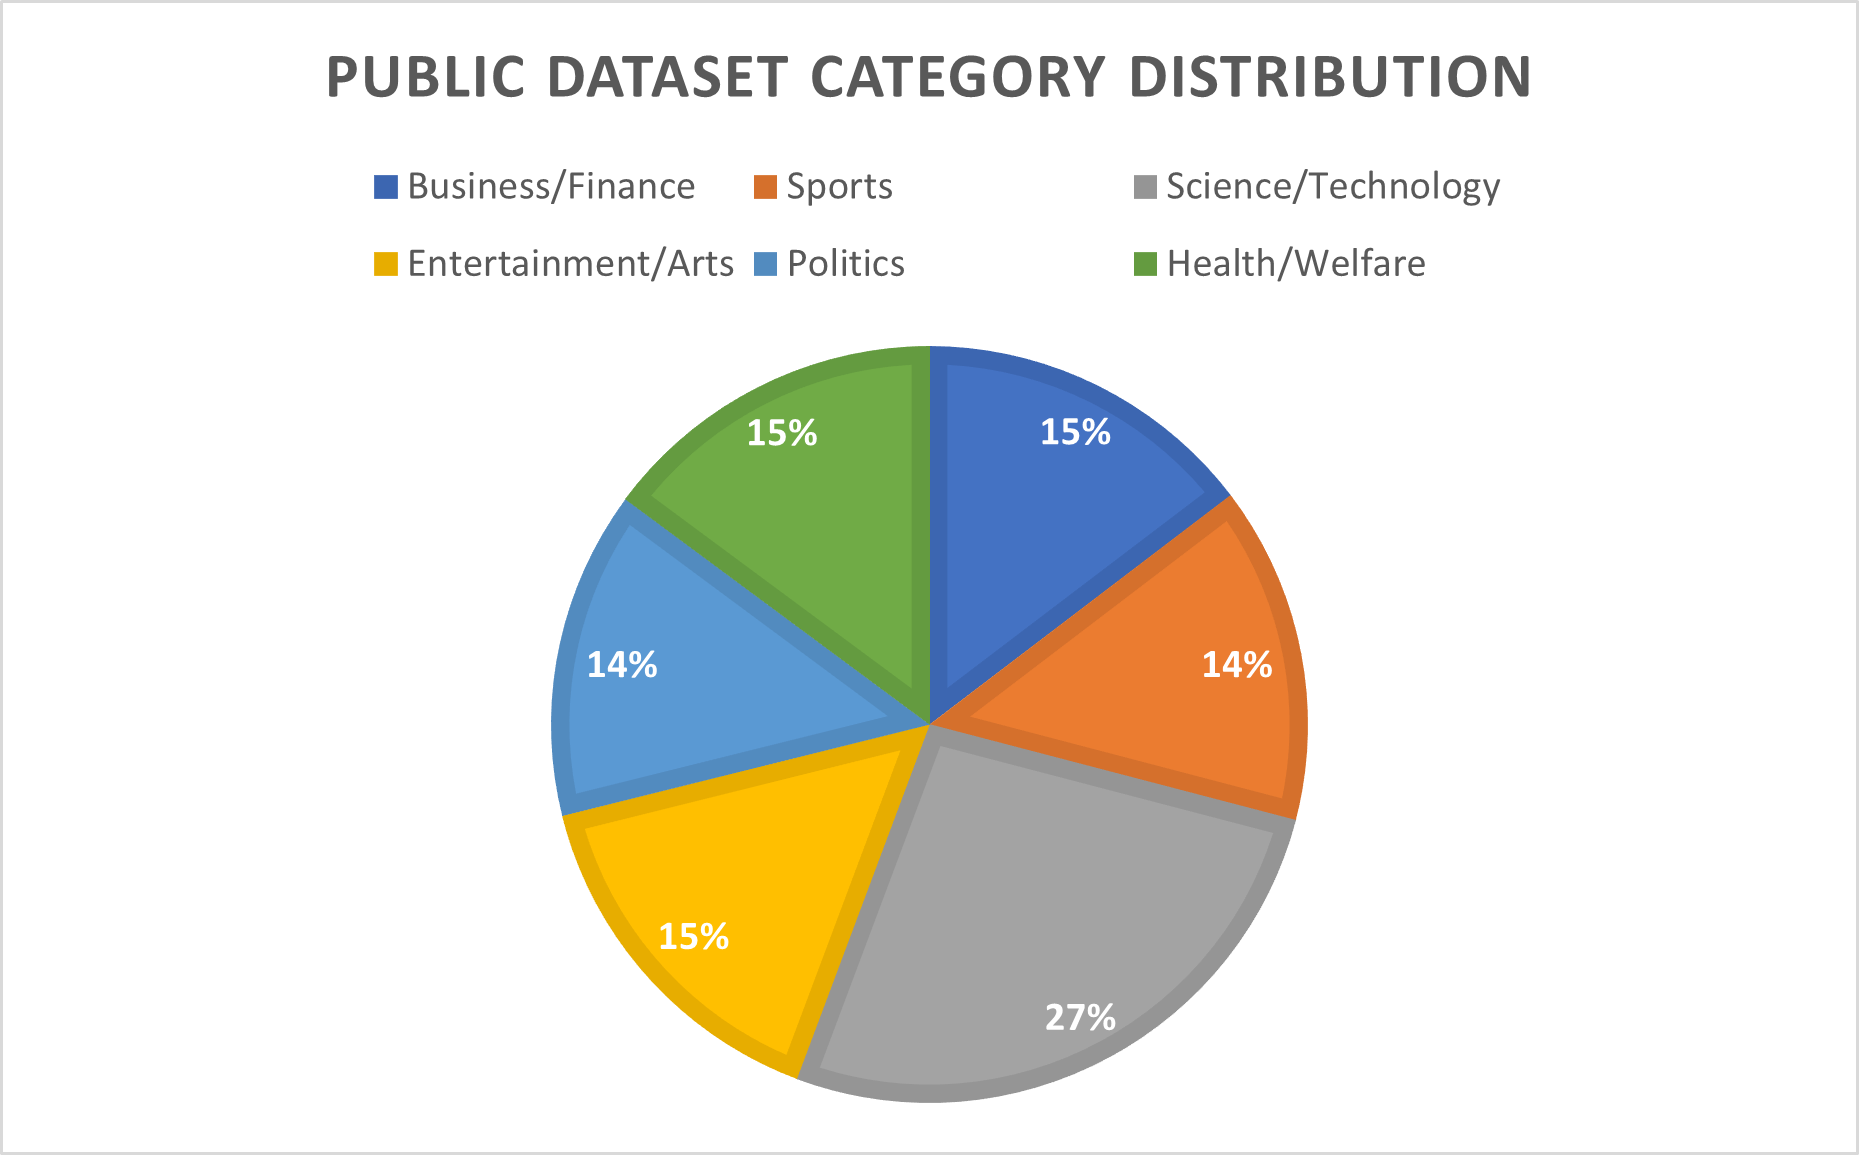
\includegraphics[width=\textwidth]{/public_category_dist.png}
\caption{The distribution of categories in the public Valurank dataset}
\label{fig:public_cat_dist}
\end{figure}

\subsubsection{Real-world data collection} \hfill \par
We collected news articles from some of the most popular online news sources across the six languages. The list of six topics used was created after considering the most common category sections in news sources across different languages, and combining similar categories which were often combined by the original sources (such as business and finance). A set of keywords relevant to each category was also generated, shown in Figure \ref{fig:dataset_category_keywords}. Each collected article was self-labelled by the source, and the articles were collected and categorised using the previously developed scraping system, with each article URL obtained and classified either through topic-specific RSS feeds or by matching the URL of article webpages with topics which match category keywords (e.g. abcnews.go.com/Sports). A complete list of data sources used is available in the appendix (link specific appendix). \par

\begin{table}[]
\begin{tabular}{ll}
\hline
\textbf{Category}           & \textbf{Keywords}                                                 \\ \hline
\textbf{Entertainment/Arts} & Entertainment, Art, Arts, Culture, Movies, Cinema, Music,         \\
\textbf{}                   & Books, Theater, Television, Dance, Celebrity                      \\
\textbf{Sports}             & Sport, Sports, Soccer, Football, Basketball, Tennis, Golf, Rugby, \\
\textbf{}                   & Motorsport, Formula 1, Physical Education                         \\
\textbf{Politics}           & Politics, Election, Parliament                                    \\
\textbf{Science/Technology} & Science, Technology, Tech, SciTech, Space, Physics                \\
\textbf{Business/Finance}   & Business, Finance, Economy, Stock exchange, Stock market, Market, \\
\textbf{}                   & Money, Investment                                                 \\
\textbf{Health/Welfare}     & Health, Welfare, Coronavirus, Pharma, Pharmacy                    \\ \hline
\end{tabular}
\caption{List of category keywords used for collecting news data. Sources which had RSS feeds or specific URL patterns with these keywords were selected for the corresponding category.}
\label{fig:dataset_category_keywords}
\end{table}

Each collected article URL was parsed using the \emph{Newspaper3k}\footnote{https://newspaper.readthedocs.io/en/latest/} library. Any article with a main body under 100 characters in length was discarded, and the article headline and body were concatenated into one text field, used for classification. Originally data was collected for 10 different languages, but only the six considered returned a sufficient number of results for model training. In the final dataset, "Business/Finance" and "Science/Technology" articles in Mandarin were downsampled in order to balance the categories, by randomly dropping articles of these categories and languages at probabilities of $p=0.75$ and $p=0.5$ respectively. \par
The distribution of articles by category and language is shown below in Table \ref{table:collectedstats} and in Figures \ref{fig:collected_cat_dist} and \ref{fig:collected_lang_dist}.

\begin{table}[]
\begin{tabular}{llllllll}
\hline
\textbf{Language}   & \multicolumn{6}{c}{\textbf{Category}}                                                                                       &                 \\ \hline
\textbf{}           & \textbf{Entertainment/} & \textbf{Sports} & \textbf{Politics} & \textbf{Science/}     & \textbf{Business/} & \textbf{Health/}   & \textbf{Total}  \\
\textbf{}           & \textbf{Arts}         & \textbf{}       & \textbf{}         & \textbf{Technology} & \textbf{Finance} & \textbf{Welfare} & \textbf{}       \\ \hline
\textbf{Mandarin}   & 511                    & 706             & 329               & 961                  & 802               & 217               & 3,526           \\
\textbf{English}    & 885                    & 682             & 435               & 607                  & 493               & 390               & 3,492           \\
\textbf{Indonesian} & 478                    & 545             & 71                & 295                  & 598               & 255               & 2,242           \\
\textbf{French}     & 342                    & 369             & 138               & 88                   & 235               & 114               & 1,286           \\
\textbf{Portuguese} & 136                    & 197             & 196               & 240                  & 232               & 167               & 1,168           \\
\textbf{Spanish}    & 203                    & 400             & 159               & 48                   & 238               & 84                & 1,132           \\ \hline
\textbf{Total}      & 2,555                  & 2,899           & 1,328             & 2,239                & 2,598             & 1,227             & \textbf{12,846}
\\ \hline
\end{tabular}
\caption{The distribution of collected news articles by language and category.}
\label{table:collectedstats}
\end{table}

\begin{figure}[h]
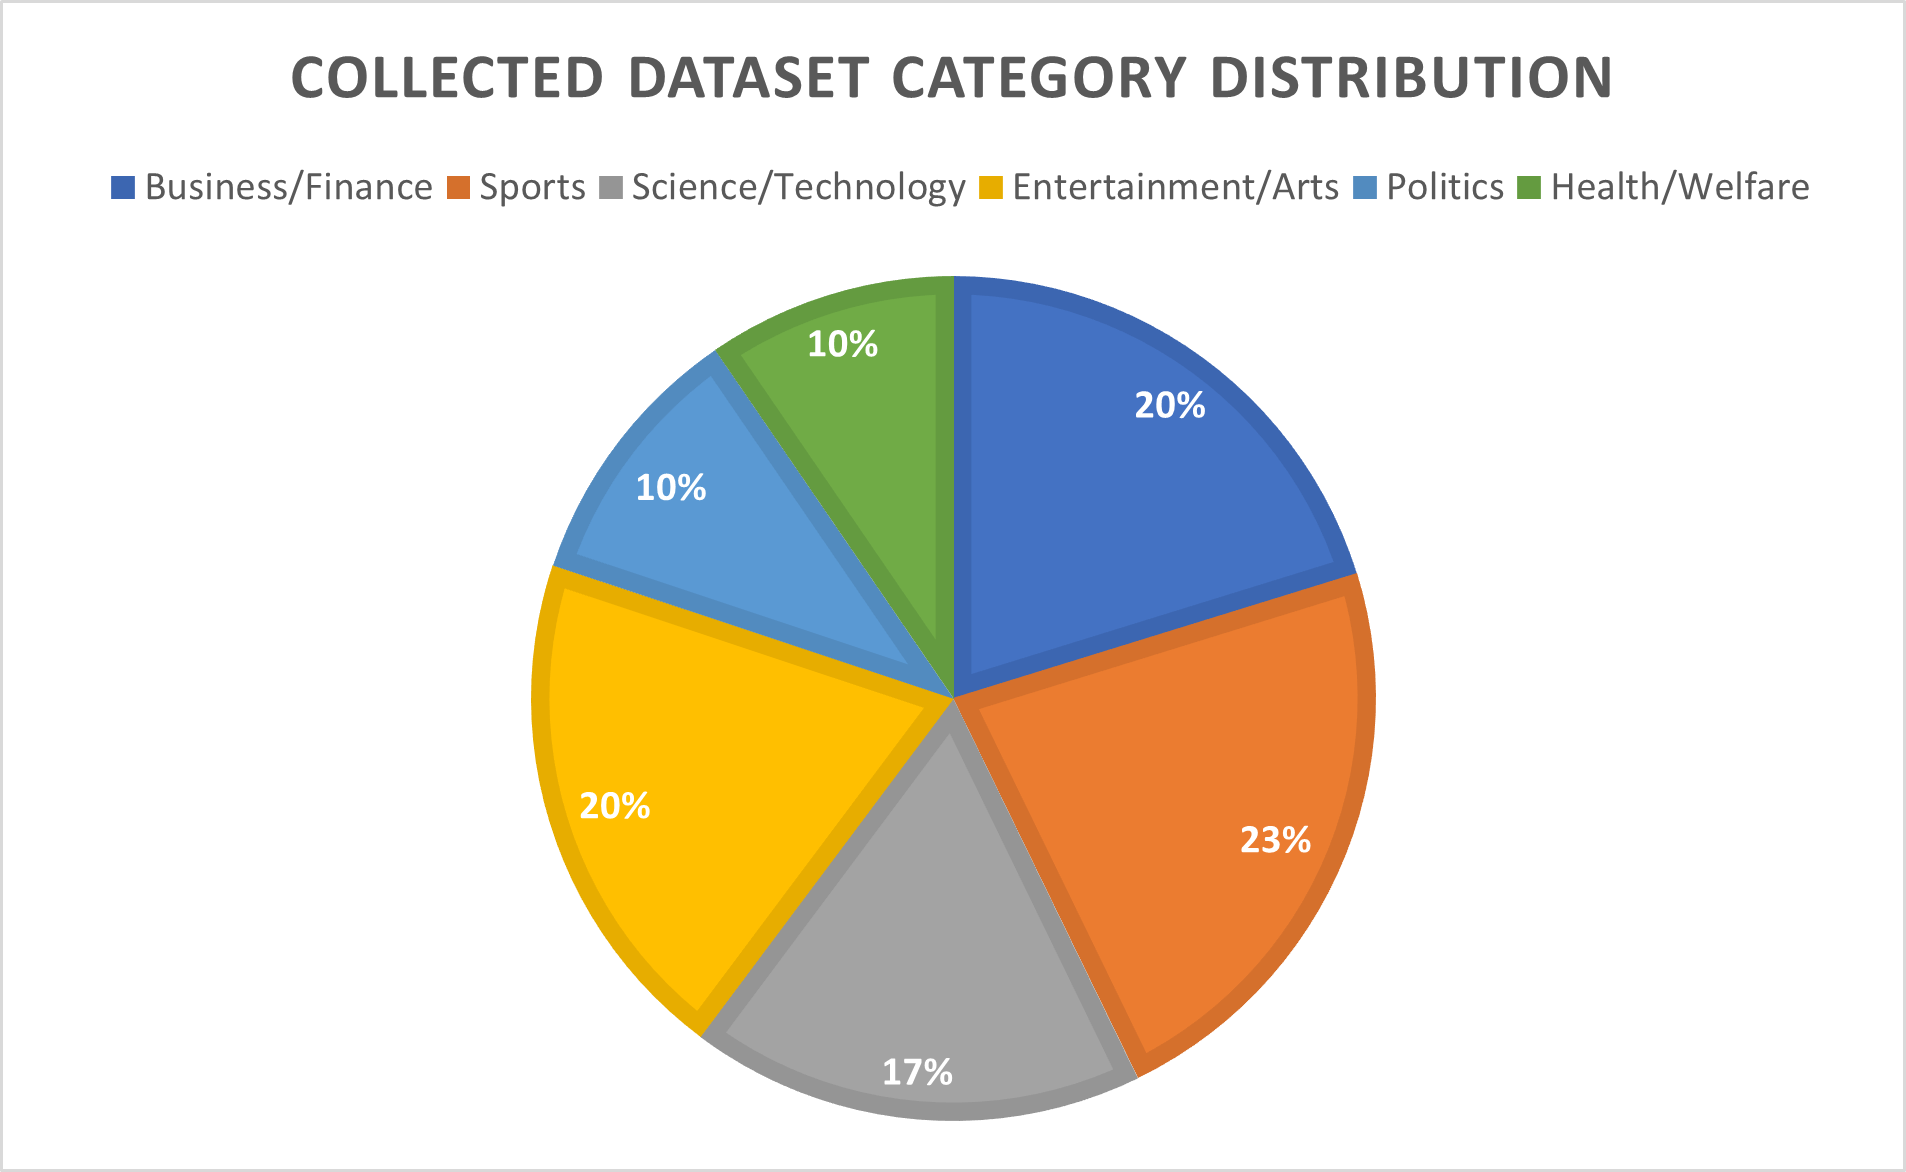
\includegraphics[width=\textwidth]{/collected_category_dist.png}
\caption{The distribution of categories in the collected dataset}
\label{fig:collected_cat_dist}
\end{figure}

\begin{figure}[h]
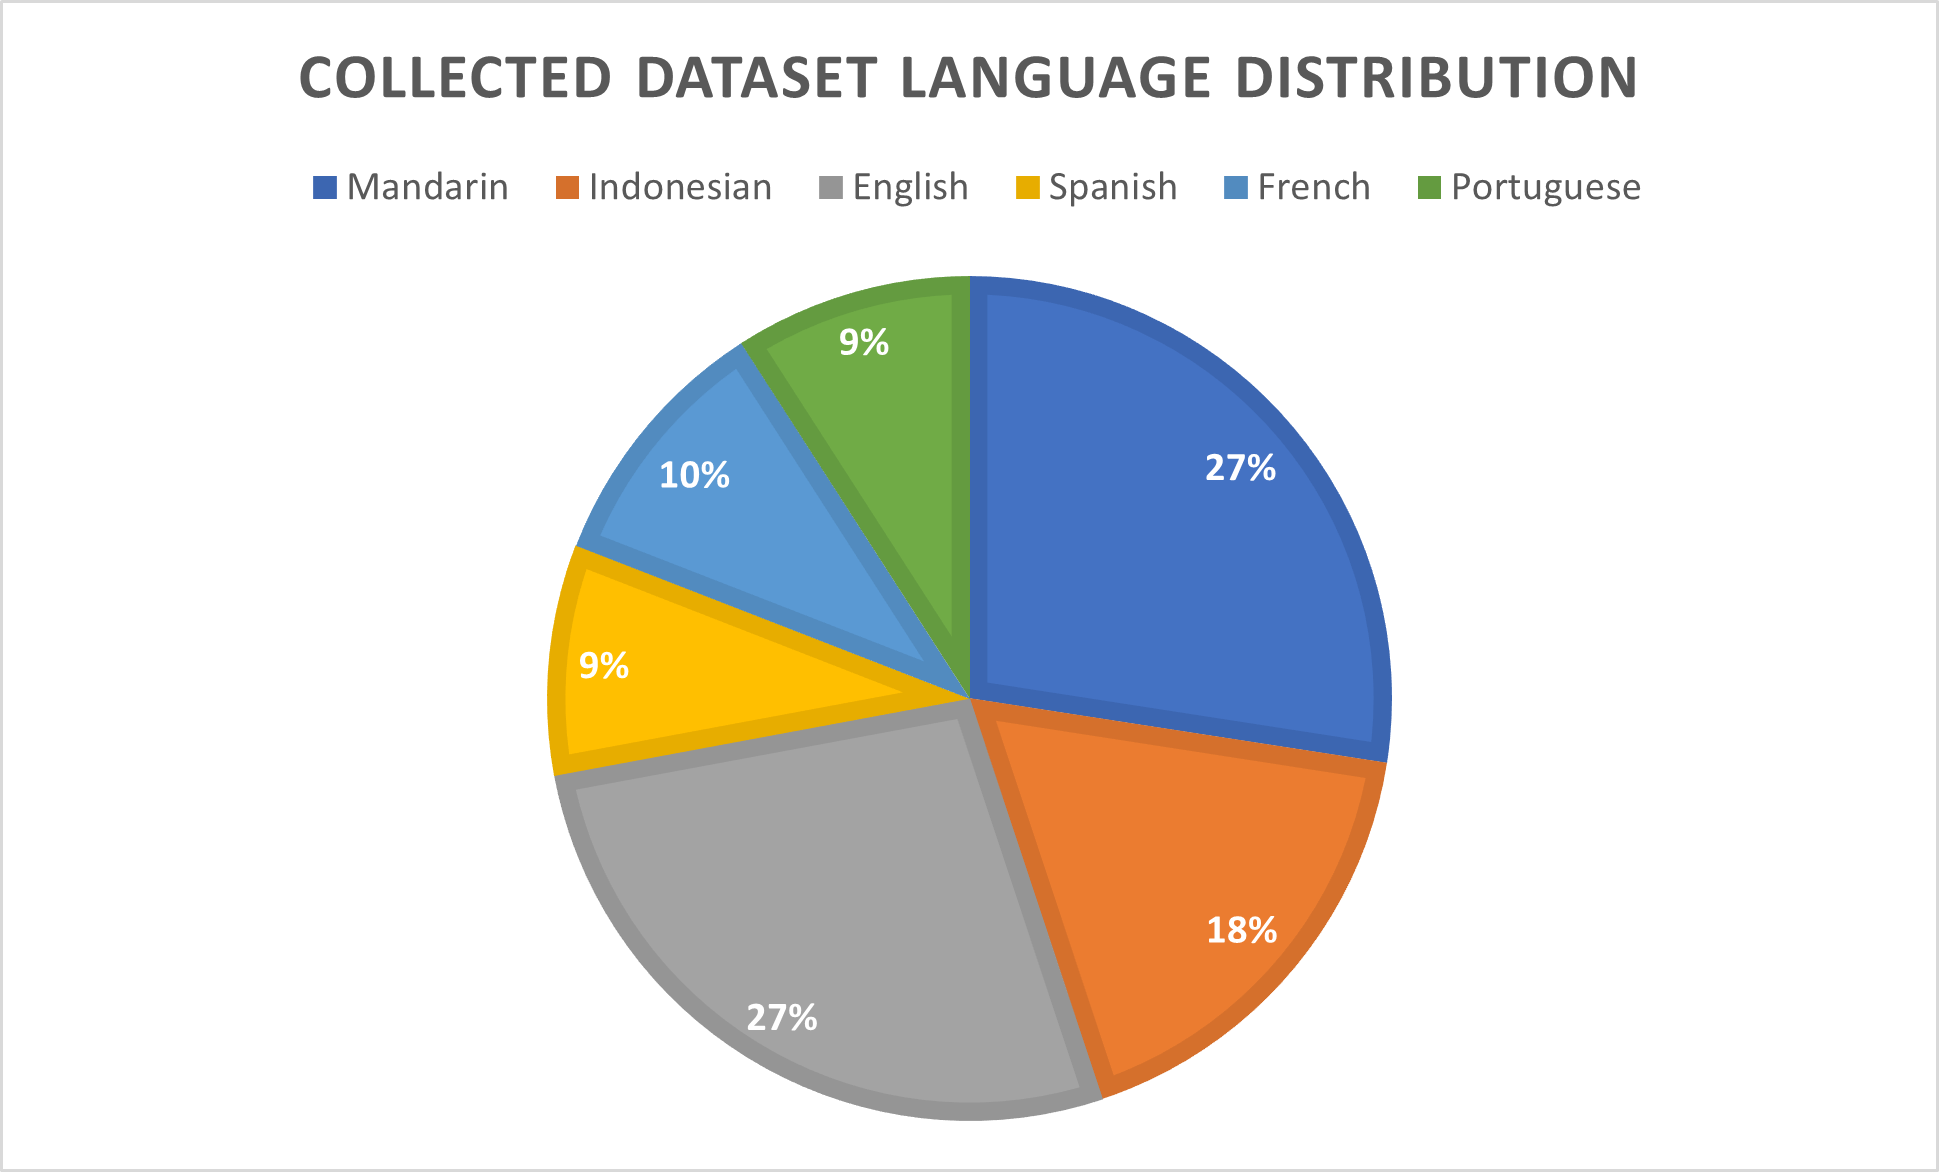
\includegraphics[width=\textwidth]{/collected_language_dist.png}
\caption{The distribution of language in the collected dataset}
\label{fig:collected_lang_dist}
\end{figure}

\subsection{Model and training choices}
\subsubsection{Multilingual models} \hfill \par
To explore the possibility of classification in real-time without the need for machine translation, only multilingual transformer models were considered. One of the most popular multilingual models is mBERT, or multilingual BERT \citep{devlin2018bert}. It was trained on the Wikipedias of the 104 languages with the most content, including the six considered here. BERT and its variations are widely used and often produce strong results in classification tasks, and the large variety of languages trained provides flexibility for potential classification of minority language sources. Research by \cite{pires2019multilingual} suggests mBERT may learn an effective language-agnostic latent space which yields impressive results when the model is evaluated on different languages than it is trained on, but this effect decreases as the languages become less structurally similar. \par
The second model being considered is XLM-RoBERTa, developed by the Facebook AI team \citep{conneau2019unsupervised}. It is trained on 2.5TB of CommonCrawl data across 100 languages, including the six considered here. It again provides a lot of coverage for minority languages and has been shown to outperform mBERT in many multilingual tasks such as named entity recognition (NER) and relation extraction \citep{li2021cross, lan2020empirical}, as well as in news classification \citep{alam2020bangla}.

\subsubsection{Baselines} \hfill \par
To test the effectiveness of machine translation upsampling, we will use the models trained on the English only public dataset as a benchmark, to measure how much (if any) accuracy increases using translation to augment the dataset. When comparing how models trained on public data transfer to collected real-world multilingual data, we can use static models which do not learn from the data as a baseline. In this case, we use two static baseline models: a model which uses stratified sampling (it samples a prediction for an input randomly, using the category densities as a probability distribution) and most common sampling (always predicts the category with the most training examples). This allows us to consider how much of what the model learns from the public data can be applied to the real-world data.

\subsubsection{Hyperparameters} \hfill \par
The hyperparameters investigated in this experiment were batch size (how many examples are used in training per backpropagation cycle), number of epochs (how many times does the model repeat the training data) and learning rate (how quickly does the model update its parameters to improve predictions). The values considered are based on the recommendations and experiments from the original BERT paper, by \cite{devlin2018bert}, and shown in Table \ref{table:hparams}. In each case, an exhaustive grid search was performed (24 trials) on the hyperparameter values and the highest accuracy model was chosen for the evaluation.

\begin{table}[]
\begin{tabular}{ll}
\hline
\textbf{Parameter}  & \textbf{Values}        \\ \hline
\textbf{Batch size} & 16, 32                \\
Number of epochs    & 2, 3, 4                \\
Learning rate       & \SI{5e-5}, \SI{4e-5}, \SI{3e-5}, \SI{2e-5}. \\ \hline
\end{tabular}
\caption{A list of hyperparameters tuned before training each model for classification. In each case, a grid search was performed with these values.}
\label{table:hparams}
\end{table}

\subsection{Data transformations}
\subsubsection{Tokenization} \hfill \par 
Each of the datasets were tokenized using the tokenizer associated with the multilingual model. multilingual BERT uses WordPiece tokenization, where each sentence is split into words by spaces or punctuation, and each word is broken into one or more subwords. Each unique subword is associated with a token ID, and input data is converted into a sequence of these token ID's, which are input into the mBERT model for classification. XLM-RoBERTa uses SentencePiece tokenization, a similar subword tokenization scheme which is lossless (it can exactly replicate the input sequence as it retains whitespace and punctuation information) and language independent \citep{kudo2018sentencepiece}. 


\subsubsection{Data splitting} \hfill \par
Because the categories in our datasets were not too imbalanced (the largest category disparity is around 2:1) we decided that data can be split randomly into a train and a test split. For each dataset, a train/test split of 80/20 (80\% training data) was used.

\subsection{Methodology}
\textbf{(TO BE COMPLETED)}
\section{Web Interface}
\textbf{(TO BE COMPLETED)}
%==================================================================================================================================
\chapter{Evaluation}

\section{Automatic web scraping system}
\textbf{(TO BE CONDUCTED)}
\section{Web Interface and Visualisations}
\subsection{Usability Testing}
(Results to be collected/analysed)
\subsection{Conclusions}
(Results to be collected/analysed)
\section{Multilingual news article classification}
\subsection{Evaluation metrics}
We will evaluate each model's performance using the  classification accuracy (which percentage of predicted categories are correct), as well as its weighted F1 score. These ratings are widely used in machine learning literature, including classification tasks \citep{alam2020bangla, al2020multiple, ranasinghe2020multilingual}. F1 score is a common metric for effectiveness in classification problems, which aims to balance precision and recall. In binary (two label) classification, precision measures the proportion of predicted positive labels (true positives and false positives) are true positives. Recall measures how many of the true positive data items (true positive and false negative predictions) were classified correctly as positive (true positive). F1 score is the harmonic mean of precision and recall, and aims to balance these metrics to favour a model which avoids false positives but also misses as few positive examples. \par
In a multiclass context, the F1 score for each possible label is calculated separately and combined. There are different methods for combining these scores, including taking a global average (micro-F1) or taking an unweighted sum of per-category averages (macro-F!). In this experiment we will use weighted F1 score, which takes a weighted average of category F1 scores based on the category weighting (the proportion of the data represented by this category). The weighted F1 score for a dataset $D$ with categories $\{c_1, c_2, ..., c_N\}$ can be calculated as:
$$Precision=\frac{TP}{TP+FP}$$ 
$$Recall=\frac{TP}{TP+FN}
$$ $$F1 \ score=2 \cdot \frac{Precision \cdot Recall}{Precision + Recall}$$
$$Weighted \ F1=\sum_{i=1}^{N}w_i \cdot F1 \ score_i \quad \quad \quad \quad w_i=\frac{|D_{d \in c_i}|}{|D|}$$

Where TP, FP and FN are the number of true positive, false positive and false negative classifications. Each experiment will be repeated for three training runs, and the mean and standard deviation of the accuracy and weighted F1 scores will be used as metrics for the effectiveness of each model.
\subsection{Classifying public data}
\subsubsection{Effectiveness of translation upsampling}  \hfill \par
Shown in Table \ref{table:backtranslation-effectiveness} are the results of training and testing the multilingual models in the original English-only and augmented translated Valurank public dataset. The results show that all models achieve very high ($>95\%$) accuracy and F1 score for the public dataset. We can also see that both models achieve an increased performance of 2-3\% on the larger translated dataset, reaching near-perfect ($>98\%$) accuracy and F1 score in both cases. In both cases, the mBERT model performs slightly better than the XLM-RoBERTa model, but there is very little difference ($<1\%$) in accuracy.

\begin{table}[]
\begin{tabular}{lllll}
\hline
\textbf{Model}   & \multicolumn{2}{l}{\textbf{English Data}} & \multicolumn{2}{l}{\textbf{Multilingual Data}} \\ \cline{2-5} 
                 & \textbf{Accuracy}    & \textbf{Weighted F1}   & \textbf{Accuracy}   & \textbf{Weighted F1}   \\ \hline 
\textbf{mBERT-base}       & \textbf{96.50$\pm$0.22}    & \textbf{96.52$\pm$0.22}          & \textbf{98.77$\pm$0.10}       & \textbf{98.77$\pm$0.10}          \\
\textbf{XLM-RoBERTa-base} & 95.66$\pm$0.37    & 95.66$\pm$0.34          & 98.70$\pm$0.00       & 98.70$\pm$0.00   
     \\ \hline
\end{tabular}
\caption{Accuracy and weighted F1 score (mean $\pm$ standard deviation) of models trained and tested on the Valurank public dataset, both in English only and translated into 5 additional languages, over 3 training runs. The most effective model for each dataset is denoted in \textbf{bold.}}
\label{table:backtranslation-effectiveness}
\end{table}

\subsubsection{Transfer of models to real-world data}  \hfill \par

Table \ref{table:transferability} shows the results of transferring the models trained on public data to real-world collected data. The trained multilingual models perform significantly better than the baseline models, but achieve significantly lower accuracies and F1 scores than when they are evaluated on the public datasets. The XLM-RoBERTa model seems to generalise more effectively on both training sets, achieving 7-9\% better accuracy and F1 score than the corresponding mBERT model. In both models, there is no significant difference in how the models perform on real-world collected data when trained on English or multilingual data.

\begin{table}[]
\begin{tabular}{lllll}
\hline
\textbf{Model}               & \textbf{English Data} &             & \textbf{Multilingual Data} &             \\ \cline{2-5} 
                             & Accuracy              & Weighted F1 & Accuracy                   & Weighted F1 \\ \hline
\textbf{Stratified Sampling} & 17.72\%$\pm$0.80     & 17.74$\pm$0.80 & 17.72\%$\pm$0.80     & 17.74$\pm$0.80            \\
\textbf{Most Common}         & 23.54\%$\pm$0.00     & 8.97$\pm$0.00 & 23.54\%$\pm$0.00     & 8.97$\pm$0.00 \\ \hline
\textbf{mBERT-base}          & 65.78\%$\pm$0.21     & 65.96$\pm$0.14         & 66.03\%$\pm$0.51        & 66.00$\pm$0.48         \\
\textbf{XLM-RoBERTa-base}    & \textbf{74.78\%$\pm$1.27}  & \textbf{74.92$\pm$1.24}        & \textbf{73.38\%$\pm$0.00}   & \textbf{73.34$\pm$0.00}        \\ \hline
\end{tabular}
\caption{Accuracy and weighted F1 score (mean $\pm$ standard deviation) of stratified sampling and most common static baseline models, as well as multilingual models trained on the Valurank public dataset (English only and translated into 5 additional languages). All models were evaluated on the collected multilingual dataset, over 3 training runs. The most effective model for each dataset is denoted in \textbf{bold.}}
\label{table:transferability}
\end{table}

\subsection{Classifying real-world data}

Table \ref{table:realworld-effectiveness} shows the results of training and testing the multilingual models on the real-world collected dataset. There is little significant difference between the two multilingual models, with XLM-RoBERTa achieving slightly higher accuracy and F1 scores of ~89.5\%. Both models achieve a lower accuracy on the collected dataset than on either of the public datasets, but perform significantly better when trained on the same dataset than on the public dataset.
Table \ref{table:confusion_matrix} shows the confusion matrix for the best performing model (XLM-RoBERTA-base) on the real-world test data. We can see that the most common misclassifications are predicting Business/Finance as Science/Technology (55 occurrences), predicting Politics as Business/Finance (48 occurrences) and predicting Science/Technology as Business/Finance (39 occurrences).  

\begin{table}[]
\begin{tabular}{lll}
\hline
\textbf{Model}   & \textbf{Accuracy} & \textbf{Weighted F1} \\ \hline
\textbf{mBERT-base}       & 87.81\%$\pm$0.24     & 87.75$\pm$0.26        \\
\textbf{XLM-RoBERTa-base} & \textbf{89.40\%$\pm$0.15}     & \textbf{89.34$\pm$0.17}                 \\ \hline
\end{tabular}
\caption{Accuracy and weighted F1 score (mean $\pm$ standard deviation) of models trained and tested on the collected multilingual dataset, over 3 training runs. The most effective model for each dataset is denoted in \textbf{bold.}}
\label{table:realworld-effectiveness}
\end{table}

\subsubsection{Confusion matrix}

\begin{table}[]
\begin{tabular}{lllllll}
\hline
\multicolumn{1}{c}{\textbf{Actual label}} & \multicolumn{6}{c}{\textbf{Predicted label}}                                                                                                                                                                                            \\ \hline
                                          & \textbf{Entertainment/}              & \textbf{Sports}                      & \textbf{Politics}                    & \textbf{Science/}                    & \textbf{Business/}                   & \textbf{Health/}                     \\
                                          & \textbf{Arts}                        & \textbf{}                            & \textbf{}                            & \textbf{Technology}                  & \textbf{Finance}                     & \textbf{Welfare}                     \\ \hline
\textbf{Entertainment/Arts}               & \cellcolor[HTML]{67FD9A}\textbf{445} & \cellcolor[HTML]{FFCCC9}6            & \cellcolor[HTML]{FFCCC9}1            & \cellcolor[HTML]{FD6864}19           & \cellcolor[HTML]{FFCCC9}4            & \cellcolor[HTML]{FFCCC9}6            \\
\textbf{Sports}                           & \cellcolor[HTML]{FFCCC9}6            & \cellcolor[HTML]{67FD9A}\textbf{558} & 0                                    & \cellcolor[HTML]{FFCCC9}3            & \cellcolor[HTML]{FFCCC9}2             & 0                                    \\
\textbf{Politics}                         & \cellcolor[HTML]{FFCCC9}5            & \cellcolor[HTML]{FFCCC9}1            & \cellcolor[HTML]{67FD9A}\textbf{196} & \cellcolor[HTML]{FD6864}11           & \cellcolor[HTML]{FE0000}48           & \cellcolor[HTML]{FD6864}15           \\
\textbf{Science/Technology}               & \cellcolor[HTML]{FFCCC9}4            & \cellcolor[HTML]{FFCCC9}3            & 0                                    & \cellcolor[HTML]{67FD9A}\textbf{385} & \cellcolor[HTML]{FE0000}39           & \cellcolor[HTML]{FFCCC9}8            \\
\textbf{Business/Finance}                 & \cellcolor[HTML]{FFCCC9}6            & \cellcolor[HTML]{FFCCC9}3            & \cellcolor[HTML]{FFCCC9}8            & \cellcolor[HTML]{FE0000}55           & \cellcolor[HTML]{67FD9A}\textbf{486} & \cellcolor[HTML]{FFCCC9}8            \\
\textbf{Health/Welfare}                   & \cellcolor[HTML]{FFCCC9}3            & \cellcolor[HTML]{FFCCC9}2            & 0                                    & \cellcolor[HTML]{FD6864}14           & \cellcolor[HTML]{FD6864}14           & \cellcolor[HTML]{67FD9A}\textbf{211} \\ \hline
\end{tabular}
\caption{Confusion matrix for the XLM-RoBERTa-base on real-world multilingual test data. The matrix shows where the prediction errors lay, and is colour coded so that deeper reds indicate more common misclassifications (the green diagonal shows correct classifications)}
\label{table:confusion_matrix}
\end{table}

\subsection{Conclusions}
Machine translation of news articles shows some promise as a means of upsampling annotated public data, yielding an improvement in classification accuracy and F1 score over training on the monolingual dataset (as shown in Table \ref{table:backtranslation-effectiveness}. For smaller datasets, this could be an effective way of synthesising much more training data to allow multilingual models to learn more effectively and achieve increased performance. Future research is required to determine if machine translation is as effective on multilingual data. \par
The large increase in performance from the baseline models when the multilingual models are trained on public data and evaluated on collected data (as shown in Table \ref{table:transferability}) suggests that the multilingual models have learned some patterns which still apply to real-world data. The decrease in accuracy and F1 score when generalising to real-world data is likely due to the differences in how news articles are categorised and written across languages. Even when translated into multiple other languages, the public dataset only captures the writing and categorisation conventions of English-language news and the exact translations do not generalise effectively to news sources in other languages. This suggests that for effective classification of news in minority languages, effort should be taken to obtain training data which is written in the language instead of relying on machine translation. \par
While performance on real-world datasets (shown in Table \ref{table:realworld-effectiveness}) remains high (~89\% accuracy) there is a significant decrease in performance in the models from the public dataset evaluation (shown in table \ref{table:backtranslation-effectiveness}. This is likely because real-world data is less simple to sort into one category than most publicly annotated data: category boundaries are often not clear and even human annotators may disagree on classifications, many articles could be considered to fit into multiple categories and some are even given multiple categories by the original news source. The model performs very well on Sports articles, where there is less overlap with other categories and hence less ambiguity, but often confuses Business/Finance, Politics and Science/Technology articles. In real-world articles, these subject areas often overlap: many political decisions affect the economy, and technology is often a topic of political debate. Future research could consider a more appropriate task for news article classification, such as multiclass classification with more labels, using human-annotated data.

\section{Project Limitations}
\subsection{News article classification}
Due to the lack of public labelled data for news article topic classification in many languages, in order to consider this task in a multilingual setting it was necessary to collect my own public data using RSS feeds and web scraping. The data collected is not annotated or reviewed by a human, and instead solely relies on the tagging of the news sources being used. This means that training data may be mislabelled or contain errors, and results achieved through experiments using these data may not be as valid as results obtained from manually annotated data. \par
Research by \cite{wu2020all} suggests that multilingual BERT is less effective in transferring its results to low-resource languages, and pre-training on a multilingual task instead of masked language modelling (MLM) would produce a better model for language transfer. Due to limited resources and time, this pre-training was not possible in this evaluation.

%==================================================================================================================================
\chapter{Conclusion}    
\textbf{(TO BE COMPLETED)}
\section{Project Summary}
\section{Future Work}
%==================================================================================================================================
%  APPENDICES  
\begin{appendices}
\textbf{(TO BE ADDED)}
\end{appendices}

%==================================================================================================================================
%   BIBLIOGRAPHY   
\bibliographystyle{abbrvnat}
\bibliography{l4proj}

\end{document}
